\documentclass[11pt]{article}

\usepackage[margin=1in]{geometry}
\usepackage[T1]{fontenc}
\usepackage[utf8]{inputenc}
\usepackage[english]{babel}

\usepackage{setspace}
\usepackage{amsmath, amssymb, amsfonts}
\usepackage{graphicx}
\usepackage{booktabs}
\usepackage{longtable}
\usepackage{array}
\usepackage{tabularx}
\usepackage{threeparttable}
\usepackage{float}
\usepackage{caption}
\usepackage{subcaption}
\usepackage{pdflscape}
\usepackage{multirow}
\usepackage{hyperref}
\usepackage{xurl}
\usepackage{chngcntr}
\usepackage{placeins}

\captionsetup[table]{font=small,labelfont=bf,justification=raggedright,singlelinecheck=false}

\newcommand{\tablepdf}[4]{%
\begin{table}[p]
\centering
\captionsetup{justification=raggedright,singlelinecheck=false}
\caption{#1}
\label{#2}
\caption*{\footnotesize #3}
\vspace{0.5em}
\includegraphics[width=\textwidth,height=0.86\textheight,keepaspectratio]{#4}
\end{table}
}

\newcommand{\apptablepdf}[4]{%
\begin{table}[H]
\centering
\captionsetup{justification=raggedright,singlelinecheck=false}
\caption{#1}
\label{#2}
\caption*{\footnotesize #3}
\vspace{0.5em}
\includegraphics[width=\textwidth,height=0.86\textheight,keepaspectratio]{#4}
\end{table}
}

\title{Measuring AI-Washing in Corporate Disclosures}
\author{Soheil Khodadadi \and Kuntara Pukthuanthong \and Thomas Walker}
\date{April 2026}

\begin{document}

\maketitle

\begin{abstract}
Artificial intelligence has become a prominent theme in corporate disclosure, yet it is difficult for investors to distinguish statements that reflect genuine implementation from those that primarily amount to narrative positioning. We classify AI-related sentences in annual 10-K filings as actionable, speculative, or irrelevant, validate this disclosure layer against subsequent AI patenting, and combine disclosure composition with contemporaneous patent weakness to construct PatentMismatch, a scalable, audited measure of AI-washing. In our 2016--2025 sample of U.S. public firms, PatentMismatch rises sharply in the post-2022 period and characterizes 41.5\% of AI-talking firm-years in 2024 and 42.1\% in 2025. Markets do not appear to fully discipline this at the filing date. Instead, the stronger correction emerges after disclosure, where a long--short strategy that buys firms with more credible AI disclosure and shorts mismatch firms earns its strongest return over the subsequent quarter, with an equal-weight alpha of 0.93\% per month, or about 11.2\% annualized. The cross-sectional valuation effects are stronger outside the largest firms. Actionable AI language aligns more closely with subsequent AI patenting than speculative language, and low-credibility disclosure predicts weaker future AI patent output. The evidence suggests that AI-washing is economically relevant both because it departs from later technological realization and because markets do not appear to price that gap immediately.
\end{abstract}

\noindent\textbf{Keywords:} Artificial intelligence; AI-washing; Corporate disclosure; 10-K filings; Textual analysis; Innovation; Patents

\noindent\textbf{JEL classifications:} D82, G14, M41, O31, O32

\section{Introduction}
Artificial intelligence now occupies a central place in corporate disclosure, yet the informational content of that language remains difficult to evaluate ex ante. AI-related investments have real implications for product innovation, operating efficiency, and firm growth (Babina et al., 2024; Cao et al., 2024), and investors appear to respond to AI narratives in corporate filings rather than treating them as generic boilerplate (Basnet et al., 2025). At the same time, the recent expansion of AI-related language in annual reports has outpaced the ability of outside investors to verify which disclosures reflect implemented technological capability and which primarily reflect narrative positioning. In our sample, more than 40\% of AI-talking firm-years in both 2024 and 2025 are classified as PatentMismatch firm-years, meaning that the filing language appears low in credibility while contemporaneous AI patenting remains weak. That pattern is difficult to reconcile with a view in which the recent surge in AI disclosure is, on average, a transparent reflection of the underlying implementation.

The fundamental economic issue is not unique to AI. In disclosure settings where implementation is difficult to verify in real time, communication can be informative without being tightly constrained by realized action. That logic is familiar from both disclosure theory and the empirical washing literature. Signaling models emphasize that communication is informative only when lower-quality senders cannot cheaply mimic higher-quality ones (Spence, 1973; Seidmann \& Winter, 1997), while empirical work in adjacent domains shows that public claims can move ahead of later observable conduct when the topic is salient and externally valued (Delmas \& Burbano, 2011; Kim \& Lyon, 2015; Lyon \& Montgomery, 2015; Baker et al., 2024). Clearly, AI-related disclosures belong to that class of problems. The underlying activity is technologically consequential, highly visible, and often difficult for investors to verify contemporaneously, making the credibility of the narrative itself an empirical question rather than a rhetorical one.

Recent work has begun to study AI communication more directly, and the closest papers provide the immediate empirical starting point for the present design. Basnet et al.~(2025) show that investors respond differently to actionable and speculative AI language in 10-K business descriptions, while Cao et al.~(2024) show that AI disclosure contains forward-looking information about firm outcomes. Bandyopadhyay et al.~(2023) connect broader AI narratives to subsequent stock mispricing, especially among firms outside the largest size group, and more recent working-paper evidence studies the divergence between AI talk and AI walk more explicitly and traces that divergence to market pricing, institutional trading, and managerial incentives (Li, 2026; Donelson et al., 2025; Barrios et al., 2025). The open question is how far a filing-based credibility measure can be scaled and audited while still preserving the distinction between more credible and less credible AI disclosure, and whether that same construct can be taken jointly to market-pricing outcomes and later technological realization.

That unresolved problem is as much about measurement as it is about economic interpretation. The textual-analysis literature has shown for some time that corporate language can contain information about later fundamentals, returns, and operating outcomes, but it has also shown how sensitive these inferences are to the way language is measured. Forward-looking statements in filings predict subsequent fundamentals (Li, 2010), disclosure language contains information beyond reported numbers (Davis et al., 2012), and textual measures in finance require domain-specific construction rather than imported dictionaries or generic sentiment tools (Loughran \& McDonald, 2011, 2016). Within innovation settings, richer text measures capture meaningful variation in firm-level technological activity and forecast subsequent patenting and performance (Bellstam et al., 2021), while public disclosure improves how markets interpret innovation-related assets (Kim \& Valentine, 2023). The question here is therefore not simply whether firms mention AI more often. It is whether the composition of that language isolates a subset of disclosures that are systematically less aligned with contemporaneous implementation and later technological realization.

Against that backdrop, we study annual 10-K filings of U.S. public firms from 2016 to 2025 and classify AI-related sentences as actionable, speculative, or irrelevant. The classification is produced by a scalable audited pipeline rather than by manual coding alone, and the resulting sentence-level judgments are aggregated into firm-year measures of disclosure composition, including the AS ratio and PatentMismatch. The latter combines low-credibility disclosure composition with weak contemporaneous AI patenting, thereby isolating a subset of AI-talking firm-years in which the narrative is difficult to reconcile with contemporaneous technological output. That same disclosure layer is then linked both to subsequent AI patent outcomes and to market measures around and after the filing date. The design is deliberately joint: if the construct captures something real, it should be informative about later innovation, and if markets do not fully distinguish credible from non-credible disclosure at the filing date, that same construct should matter for the subsequent return path.

The empirical evidence follows a clear sequence. It begins with the sharp post-2022 rise in PatentMismatch and characterizes 41.5\% of AI-talking firm-years in 2024 and 42.1\% in 2025. However, filing-date abnormal returns provide little evidence of immediate discipline, whereas the sharper pricing pattern appears after disclosure: a long--short strategy that buys firms with more credible AI disclosure and shorts mismatch firms earns its strongest return over the subsequent quarter, with an equal-weight alpha of 0.93\% per month, or roughly 11.2\% annualized. That effect is much weaker in value-weighted specifications, suggesting that the slower correction is concentrated outside the largest firms. In that respect, the return evidence is closer to delayed incorporation than to immediate repricing and is consistent with filing-based settings in which disclosure-related information is not fully impounded at the announcement date (Cohen et al., 2020). Furthermore, the disclosure construct remains tied to later technological realization: actionable AI language aligns more closely with subsequent AI patenting than speculative language, and the AS-ratio $\times$ PatentMismatch specification predicts weaker subsequent AI patent output. The post-ChatGPT tests point in the same direction. What makes the pattern economically important is not only that low-credibility AI disclosure became widespread, but that the market appears to underreact to it even as it predicts weaker subsequent technological realization.

Basnet et al.~(2025) provide the closest filing-based starting point by showing that investors distinguish between actionable and speculative AI language in 10-K business descriptions, while Bandyopadhyay et al.~(2023) show that broader AI narratives are associated with subsequent stock mispricing, especially outside the largest firms. Li (2026) moves even closer to the present setting by studying the divergence between AI talk and AI walk and its market consequences. Building on those studies, the present paper scales the actionable--speculative distinction into a reusable audited framework for mandatory annual filings, introduces PatentMismatch as a filing-based construct that combines disclosure composition with contemporaneous patent weakness, and uses that construct to connect low-credibility AI disclosure both to slower market correction and to weaker subsequent AI patent realization. The contribution therefore lies in identifying which subset of filing-based AI narratives appears least credible and in showing that this subset is economically important in both prices and later technological realization.

The remainder of the paper proceeds as follows. Section 2 reviews the related literature. Section 3 describes the data, the measurement pipeline, and the empirical design. Section 4 presents the main results. Section 5 concludes.

\section{Literature Review}
In accounting and finance, disclosure has long been viewed not as a neutral release of information, but as an equilibrium object shaped by information asymmetry, proprietary costs, reputational concerns, and the strategic incentives surrounding communication (Healy \& Palepu, 2001; Verrecchia, 2001; Beyer et al., 2010). That logic becomes especially important when the underlying activity is difficult to verify in real time. Signaling models make the point formally: communication is most informative when higher-quality senders can distinguish themselves through statements or actions that lower-quality senders cannot cheaply mimic (Spence, 1973; Seidmann \& Winter, 1997). In settings where implementation is costly but language is inexpensive, disclosure can remain informative without cleanly mapping into realized action. It is precisely in such settings that the distinction between substantive and rhetorical disclosure becomes economically meaningful.

Empirical work on washing sharpens that intuition. Studies of greenwashing show that public claims about sustainability can diverge from realized behavior when firms face strong incentives to appear aligned with socially valued goals (Delmas \& Burbano, 2011; Kim \& Lyon, 2015; Lyon \& Montgomery, 2015). Marquis et al.~(2016) document how selective disclosure can produce the appearance of transparency even when the underlying record is weaker, and Hummel and Schlick (2016) show that disclosure quality rather than disclosure quantity governs whether reporting tracks actual performance. Baker et al.~(2024) bring the same logic to diversity-related disclosure and show that public claims can outpace subsequent workforce outcomes. These studies clearly define the economic problem . When a topic is salient, externally valued, and only imperfectly verifiable, firms may have incentives to use language more aggressively than the underlying implementation record would justify.

A parallel line of work now studies AI communication more directly. Basnet et al.~(2025) show that investors respond differently to actionable and speculative AI language in 10-K business descriptions, while Cao et al.~(2024) show that AI disclosure contains forward-looking information about firm outcomes. Bandyopadhyay et al.~(2023) connect a broader AI narrative measure to subsequent stock mispricing, particularly outside the largest firms, and recent working-paper evidence studies divergence between AI talk and AI walk more explicitly (Li, 2026; Donelson et al., 2025; Barrios et al., 2025). The literature is therefore moving beyond raw mention counts and toward the credibility of AI-related language itself. However, the empirical design choices differ. Some studies focus on manual classification, some on broader narrative exposure, and some on talk--walk divergence measured outside mandatory annual filings. What remains comparatively underdeveloped is a filing-based framework that can be audited, scaled, and reused while preserving the distinction between more credible and less credible AI disclosure inside annual 10-Ks.

Measurement is material since the textual-analysis literature has repeatedly shown that corporate language is informative only when measured in a way that fits the institutional setting. Forward-looking language in filings predicts later fundamentals (Li, 2010), earnings-press-release language contains information beyond the quantitative surprise itself (Davis et al., 2012), and textual measures in finance are highly sensitive to how the underlying vocabulary is constructed (Loughran \& McDonald, 2011, 2016). At the same time, tone and wording can be managed strategically rather than passively reflecting fundamentals (Huang et al., 2014). The implication is not that narrative disclosure is unreliable. The empirical content of narrative disclosure depends on whether the measure isolates the relevant dimension of the language rather than collapsing everything into a broad mention count. That point is especially important in an AI setting, where generic references, aspirational language, and implemented uses can all appear in the same filing while conveying very different information.

The innovation literature points in the same direction. Bellstam et al.~(2021) show that richer textual measures capture meaningful differences in firm-level innovation and forecast subsequent patenting and performance, while Kim and Valentine (2023) show that public disclosure improves how markets interpret innovation-related assets. Those papers justify the two sides of the current design. Filing language can contain information about later technological activity. However, not all ways of describing that language will be equally informative. The purpose of this paper hence is to identify whether the composition of that language isolates a subset of disclosures that are systematically less aligned with contemporaneous implementation and subsequent technological realization. That is the narrower question around which this paper is organized.

\section{Data and Methodology}
\subsection{Sample construction and data sources}

We combine four linked data layers:  10-K annual filings, AI-related patent outcomes, market data, and firm-level accounting controls. The disclosure layer is built from firms' annual 10-K filings, which provide the sentence-level corpus used to measure AI-related language. The innovation outcomes are constructed from AI-related patent grants drawn from USPTO/PatentsView and matched to public firms through a CIK--ticker--GVKEY--assignee crosswalk. Market outcomes are drawn from CRSP and are used for filing-date abnormal-return tests and post-filing return analyzes. Firm characteristics and annual controls come from Compustat.

The main empirical backbone is an ever-speaker annual panel covering 2016--2025. A firm enters this panel if it mentions AI at least once during the sample window, and the panel then retains all available annual observations for that firm, including years with zero AI-related disclosure. This design is important because it preserves the non-speaking years needed to distinguish prior, contemporaneous, and later outcomes on a common annual scaffold. The ever-speaker panel contains 50,840 firm-year observations across 5,084 firms.

Within this annual backbone, 13,777 firm-years contain at least one classified AI sentence, and the linked filing-event sample contains 7,355 annual filing events across 2,753 firms, of which 7,342 have usable CAR[$-1,+1$] returns and 7,098 have usable BHAR[$+2,+63$] outcomes.

This annual backbone supports two linked outcome families. The first is a set of later innovation outcomes based on AI-related patenting. The second is a set of market-based outcomes built around the 10-K filing date and the post-filing return path. The market tests use CRSP-linked filing-event samples and monthly return panels, while the innovation tests use the annual firm-year panel. Not every empirical block uses exactly the same observations. Sample sizes change mechanically because some specifications require AI-talking firm-years, some require lead or lag patent outcomes, and some require complete cases on the annual control set. The filing-date event-study tests also impose CRSP availability and event-window requirements. Appendix Table~\ref{tab:appendix_attrition} reports the resulting attrition across the main empirical blocks.

We therefore do not rely on a single estimation sample. Instead, we use a common filing-based disclosure layer, constructed once, and then links that layer to separate annual and event-time outcomes. This structure is useful for the current research design because it allows the same disclosure-credibility construct to be evaluated in two ways: by asking whether it predicts later AI-related innovation, and whether markets appear to distinguish more credible from less credible AI disclosure when the 10-K is released.

\subsection{Sentence extraction and AI-language classification}

We segment each filing into sentences and remove duplicate blocks, tables, headers, and other clearly non-narrative content. We then identify AI-related sentences using a versioned keyword dictionary that includes terms such as ``artificial intelligence,'' ``machine learning,'' ``deep learning,'' ``neural network,'' ``natural language processing,'' ``computer vision,'' ``robotic process automation,'' ``large language model,'' and ``generative AI.'' Each retained sentence is keyed to the firm and fiscal year of the filing.

The core measurement step is a three-way sentence classification. Actionable sentences describe concrete AI deployments, embedded workflows, internal tools, or productized uses. Speculative sentences refer to AI in aspirational, exploratory, or forward-looking terms without enough operational detail to verify current implementation. Irrelevant sentences contain generic or tangential AI references that do not speak to the firm's own capability.

The scaling pipeline is organized as three sequential gates rather than one blended procedure. First, we build a human labeling rubric and conduct an inter-rater-reliability audit on a stratified validation subset. Second, we evaluate a tuned three-stage classifier against the adjudicated labels and use that model to scale the classification across the full sentence corpus. Third, we validate the resulting firm-year measures against independently constructed AI patent outcomes. This separation matters because rubric reliability, classifier accuracy, and external validation answer different questions. In the expanded 2016--2025 sample, the classified corpus contains 147,879 AI-related sentences, including 67,080 actionable sentences, 17,900 speculative sentences, and 62,899 irrelevant sentences.

Appendix Table~\ref{tab:appendix_audit} reports the measurement audit underlying the disclosure-classification layer. The adjudicated sentence base contains 551 labeled observations, the leakage-safe training and calibration pool contains 431 observations, and the adjudicated heldout benchmark contains 120 observations. In the human--human IRR rerun, Cohen's kappa is 0.850 after adjudication of 12 disagreements. On the heldout benchmark, the selected hybrid policy attains 85.0\% accuracy, 83.6\% macro-F1, 91.7\% binary relevance, and 86.5\% actionable-versus-speculative performance.

\subsection{Firm-year disclosure measures}

Let $A_{i,t}$, $S_{i,t}$, and $I_{i,t}$ denote the number of actionable, speculative, and irrelevant AI sentences in firm $i$'s filing in year $t$. Let
\[
N_{i,t} = A_{i,t} + S_{i,t} + I_{i,t}
\]
denote total AI-related sentences.

The broad disclosure-intensity measure is
\[
\mathrm{AI Focus}_{i,t} = \log(1 + N_{i,t}).
\]

We also define disclosure-type indicators. $\mathrm{ActionableDisclosure}_{i,t}$ equals one if $A_{i,t} > 0$ and zero otherwise. $\mathrm{SpeculativeOnly}_{i,t}$ equals one if $S_{i,t} > 0$ and $A_{i,t} = 0$. These two indicators separate firm-years with any concrete AI implementation language from firm-years that mention AI only in speculative terms.

For descriptive work and companion specifications, we also retain the sentence counts and their log transforms. To summarize credibility tilt, we define
\[
\mathrm{ActionableShare}_{i,t} = \frac{A_{i,t}}{A_{i,t} + S_{i,t}},
\qquad
\mathrm{SpecShare}_{i,t} = \frac{S_{i,t}}{A_{i,t} + S_{i,t}},
\]
for firm-years with $A_{i,t} + S_{i,t} > 0$, and zero otherwise. We also define
\[
\mathrm{CredAI}_{i,t} = z(A_{i,t}) - z(S_{i,t}),
\]
where $z(\cdot)$ denotes within-sample standardization.

The main metric used in the interaction specifications is the actionable-to-speculative (AS) ratio
\[
AS_{i,t} = \log\left(1 + \frac{A_{i,t}}{1 + S_{i,t}}\right).
\]

This stabilized ratio rises as AI language becomes more actionable and falls as speculative language becomes more prominent, while remaining defined when $S_{i,t} = 0$. In the empirical analysis, the AS ratio is the primary disclosure-credibility regressor, while $\mathrm{SpecShare}_{i,t}$ and $\mathrm{CredAI}_{i,t}$ are secondary companion measures.

Note that the ever-speaker panel retains many zero-disclosure years by construction. For those firm-years, the intensity and composition measures equal zero. This is a feature of the design, not a data error: those restored zero years make the timing comparisons interpretable.

\subsection{Outcome families: patents, returns, valuation, and financing}

The empirical design evaluates the disclosure-credibility construct against two linked outcome families. The first consists of later AI-related innovation outcomes. The second consists of market-based and capital-market outcomes around and after the annual 10-K filing. The central idea is that the same filing-based disclosure measure should be informative both about later technological realization and about whether markets distinguish more credible from less credible AI disclosure when the filing is released.

The innovation outcomes are built from the matched AI patent series described above. The main patent outcome is $\log(1+\mathrm{AIPatents}_{i,t+h})$, where $h \in \{-2,-1,0,+1,+2\}$ indexes calendar-time horizons relative to the disclosure year. These outcomes are used to validate the disclosure construct against later observable technological output and to distinguish backward-looking, contemporaneous, and forward-looking timing patterns.

The market-based outcomes are constructed from CRSP return data linked to annual 10-K filing dates. For short-window market reaction tests, we use filing-date cumulative abnormal returns computed from daily stock returns net of the value-weighted market return. The baseline filing-date window is $[-1,+1]$ trading days around the filing date, and the current event-study block also includes event-time plots over the daily window from trading day $-2$ to trading day $+2$. For slower price adjustment, we construct post-filing buy-and-hold abnormal returns beginning on trading day $+2$ so that the immediate filing window is excluded. These post-filing windows are evaluated over horizons of 1, 3, 6, and 12 months, with the strongest current results centered on the quarterly window.

To complement the event-level return tests, we also form calendar-time long--short portfolios using the latest available filing signal for each stock-month. In these portfolios, the long leg holds non-mismatch AI filers and the short leg holds mismatch AI filers. We evaluate both equal-weight and value-weight implementations over alternative holding windows and estimate market alpha as the intercept from regressions of long--short monthly returns on the value-weighted market return. These portfolio tests are useful because they summarize whether any post-filing return differential is concentrated in smaller names or survives after market adjustment.

The final outcome block is annual and cross-sectional rather than event-time based. These tests use valuation and financing outcomes constructed from linked market features and accounting data. The valuation side includes log market-capitalization-to-assets and a log Tobin's-$Q$ proxy. The financing side includes the next-year change in shares outstanding and an indicator for substantial next-year share growth. These consequence tests are strongest outside the largest firms, so the main-text specification uses the non-big subsample while fuller variants remain available as supporting material.

\subsection{PatentMismatch construction and determinants}

The central low-credibility disclosure construct is PatentMismatch. The indicator is defined at the firm-year level and can take the value one only in AI-talking firm-years. Intuitively, PatentMismatch identifies firm-years in which the filing narrative appears weak in credibility relative to the firm's contemporaneous AI implementation record. The construct therefore combines a language-side signal with a same-year technology-side signal rather than relying on either one alone.

Formally, $\mathrm{PatentMismatch}_{i,t}=1$ when firm-year $(i,t)$ is an AI-talking year, $AS_{i,t}$ falls in the bottom quartile of the year-$t$ AI-talking distribution or $\mathrm{SpecShare}_{i,t}$ lies in the top quartile of that same distribution, and contemporaneous $\log(1+\mathrm{AIPatents}_{i,t})$ is below the year-$t$ industry-year mean of $\log(1+\mathrm{AIPatents})$; otherwise $\mathrm{PatentMismatch}_{i,t}=0$. The low-credibility gate therefore uses an OR rule across the AS ratio and speculative share, while the patent-weakness condition must also be satisfied. Outside AI-talking firm-years, the indicator is coded as zero.

This timing discipline is important for interpretation. PatentMismatch uses only year-$t$ information: the composition of disclosure in the filing year and contemporaneous patent weakness measured relative to the year-$t$ industry benchmark. It does not use future patent outcomes in its construction. That design is intended to avoid mechanical circularity when the construct is later related to post-filing returns or to future AI patenting.

The role of PatentMismatch differs across the empirical blocks. In the annual innovation-validation regressions, it enters either directly or interacted with the AS ratio to test whether lower-credibility AI disclosure predicts weaker subsequent AI patent realization. In the filing-date and post-filing market tests, it serves as the main low-credibility disclosure indicator used to distinguish firms whose AI language appears least aligned with contemporaneous implementation. In the annual valuation and financing tests, it is used to ask whether these same low-credibility firm-years are associated with different market valuation or financing outcomes.

The construct also supports a separate cross-sectional determinants exercise. In those appendix specifications, the dependent variable is either an indicator for whether a firm records at least one PatentMismatch incident during 2016--2025 or the share of AI-talking years flagged as mismatch over the same period. Baseline firm characteristics are measured in 2016, and the determinants block is intended to describe where mismatch is concentrated rather than to establish a causal mechanism.

\subsection{Empirical specifications}

The empirical design is organized in four blocks: innovation-validation regressions, filing-date event tests, post-filing return tests, and annual valuation/financing tests. All specifications use the same underlying disclosure layer, but the unit of observation and timing structure differ across blocks.

First, to validate the disclosure measures against later technological output, we estimate annual panel regressions of the form
\[
\log(1+\mathrm{AIPatents}_{i,t+h})
=
\alpha_h + \beta_h \mathrm{Narrative}_{i,t} + X_{i,t}'\theta_h + \gamma_i + \gamma_t + \varepsilon_{i,t+h},
\]
where $h \in \{-2,-1,0,+1,+2\}$ and $\mathrm{Narrative}_{i,t}$ is alternatively $\mathrm{AI Focus}_{i,t}$, $\mathrm{ActionableDisclosure}_{i,t}$, $\mathrm{SpeculativeOnly}_{i,t}$, or the AS ratio interacting with $\mathrm{PatentMismatch}_{i,t}$. The baseline control set includes log assets, leverage, cash/assets, R\&D/assets, CAPX/assets, ROA, sales growth, and employees. The main specifications include firm and year fixed effects, with companion columns using industry$\times$year fixed effects and standard firm-level clustering. These regressions are predictive timing tests rather than causal designs; their purpose is to determine whether different forms of AI disclosure line up differently with prior, contemporaneous, and later AI patenting.

Second, to study immediate market reaction, we estimate filing-level event regressions of the form
\[
CAR_{i,f,[a,b]}
=
\alpha + \beta_1 \mathrm{PatentMismatch}_{i,t}
+ \beta_2 AS_{i,t}
+ \beta_3 \mathrm{AI Focus}_{i,t}
+ X_{i,t-1}'\theta + \delta_{j} + \lambda_{\tau} + \varepsilon_{i,f},
\]
where $CAR_{i,f,[a,b]}$ is the market-adjusted cumulative abnormal return for firm $i$ around filing event $f$ over event window $[a,b]$, $\delta_{j}$ denotes industry fixed effects, and $\lambda_{\tau}$ denotes filing-year fixed effects. The baseline filing window is $[-1,+1]$. The event sample is restricted to AI-talking 10-K and 10-K/A filings with complete event-window returns and successful merges back to the annual disclosure panel. Standard errors are clustered at the firm level. These tests ask whether low-credibility AI disclosure is associated with different abnormal-return patterns at the filing date, conditional on lagged firm characteristics and common industry and filing-year effects.

Third, to examine slower price adjustment, we estimate post-filing abnormal-return regressions using buy-and-hold abnormal returns beginning on trading day $+2$:
\[
BHAR_{i,f,[+2,H]}
=
\alpha + \beta_1 \mathrm{PatentMismatch}_{i,t}
+ \beta_2 AS_{i,t}
+ \beta_3 \mathrm{AI Focus}_{i,t}
+ X_{i,t-1}'\theta + \delta_{j} + \lambda_{\tau} + \varepsilon_{i,f,H},
\]
where $H$ indexes the post-filing horizon. We evaluate horizons corresponding to approximately 1, 3, 6, and 12 months. We complement these regressions with calendar-time long--short portfolios that buy non-mismatch AI filers and short mismatch filers using the most recent filing signal for each stock-month. Equal-weight and value-weight portfolios are evaluated separately, and alpha is estimated as the intercept from regressing the long--short monthly return on the value-weighted market return. These tests summarize whether any filing-related return differential emerges only after the filing and whether that pattern is concentrated in smaller firms.

Fourth, to examine annual capital-market consequences, we estimate firm-year regressions of the form
\[
Y_{i,t+h}
=
\alpha + \beta_1 \mathrm{PatentMismatch}_{i,t}
+ \beta_2 AS_{i,t}
+ \beta_3 \mathrm{AI Focus}_{i,t}
+ X_{i,t}'\theta + \gamma_i + \gamma_t + \varepsilon_{i,t+h},
\]
where $Y_{i,t+h}$ is alternatively a valuation or financing outcome. The valuation outcomes include log market-capitalization-to-assets and a log Tobin's-$Q$ proxy, and the financing outcomes include next-year share growth and an indicator for substantial next-year issuance. These specifications use firm- and year fixed effects with firm-clustered standard errors. Because the cleaner patterns are concentrated outside the largest firms, the main-text version reports the non-big subsample, while broader variants are retained as supporting evidence.

Across all four blocks, the role of the disclosure variables is the same. $\mathrm{AI Focus}_{i,t}$ captures the broad intensity of the AI narrative, the AS ratio captures the composition of the disclosure, and $\mathrm{PatentMismatch}_{i,t}$ identifies firm-years in which disclosure composition and contemporaneous implementation appear misaligned. The aim is not to claim a single causal design across all outcomes. Rather, it is to evaluate whether the same filing-based construct is informative about later innovation, immediate market reaction, slower post-filing correction, and broader capital-market consequences.

\subsection{Exploratory post-ChatGPT design}

A final empirical block examines whether the disclosure-credibility patterns intensify after the public release of ChatGPT. We treat this exercise as exploratory rather than as the primary identification strategy. The release of ChatGPT sharply increased the salience of AI-related language and may have lowered the cost of inserting AI talk into annual filings, but it may also coincide with broader changes in implementation, attention, and experimentation. For that reason, the post-ChatGPT results are interpreted as suggestive evidence rather than as a clean causal estimate.

The baseline implementation defines $\mathrm{PostChatGPT}_t=1$ for the years 2023 and later and constructs treatment status from the pre-period 2018--2022. The main treatment identifies low-capability firms: firms with zero pre-period AI patents and either a low pre-period AS ratio or no pre-period actionable AI disclosure. The intuition is that these firms have the weakest ex ante evidence of AI capability yet may be the most exposed to a fall in the cost of AI-related narrative production. We also consider two alternative treatment definitions in supporting specifications: firms with high pre-period speculative intensity relative to their industry and firms with low pre-period market capitalization.

The exploratory specifications take the form of
\[
Y_{i,t}
=
\alpha_i + \lambda_t + \beta \big(\mathrm{PostChatGPT}_t \times \mathrm{Treated}_i\big) + X_{i,t-1}'\theta + \varepsilon_{i,t},
\]
where $Y_{i,t}$ is alternatively AI Focus, AS ratio, PatentMismatch, filing-date abnormal returns, or post-filing abnormal returns. The annual specifications use firm- and year fixed effects where appropriate, and the event-based outcome specifications inherit the corresponding event-study sample restrictions. The purpose of these tests is to examine whether the period after late 2022 is associated with a sharper increase in low-credibility AI disclosure among firms with weaker pre-period AI capability.

Our results show that the post-ChatGPT interaction is strongest for PatentMismatch, while the filing-date abnormal-return specification shows little evidence of a parallel market response. The pretrend diagnostics are also mixed across the outcomes, reinforcing the view that these tests are best interpreted as exploratory rather than definitive.

\section{Empirical Analysis and Results}
\subsection{The scale and timing of low-credibility AI disclosure}

We begin with a descriptive analysis. Figure~\ref{fig:mismatch_surge} shows that low-credibility AI disclosure becomes common quickly in the post-2022 period. The number of AI-talking firm-years flagged as PatentMismatch rises sharply after 2022, and the mismatch share among AI-talking firm-years reaches 41.48\% in 2024 and 42.12\% in 2025. The recent expansion of AI language in annual filings is not simply a broad increase in AI-related discussion; it is also associated with a rapid increase in the subset of firm-years in which disclosure composition appears difficult to reconcile with contemporaneous AI patenting.

\begin{figure}[p]
\centering
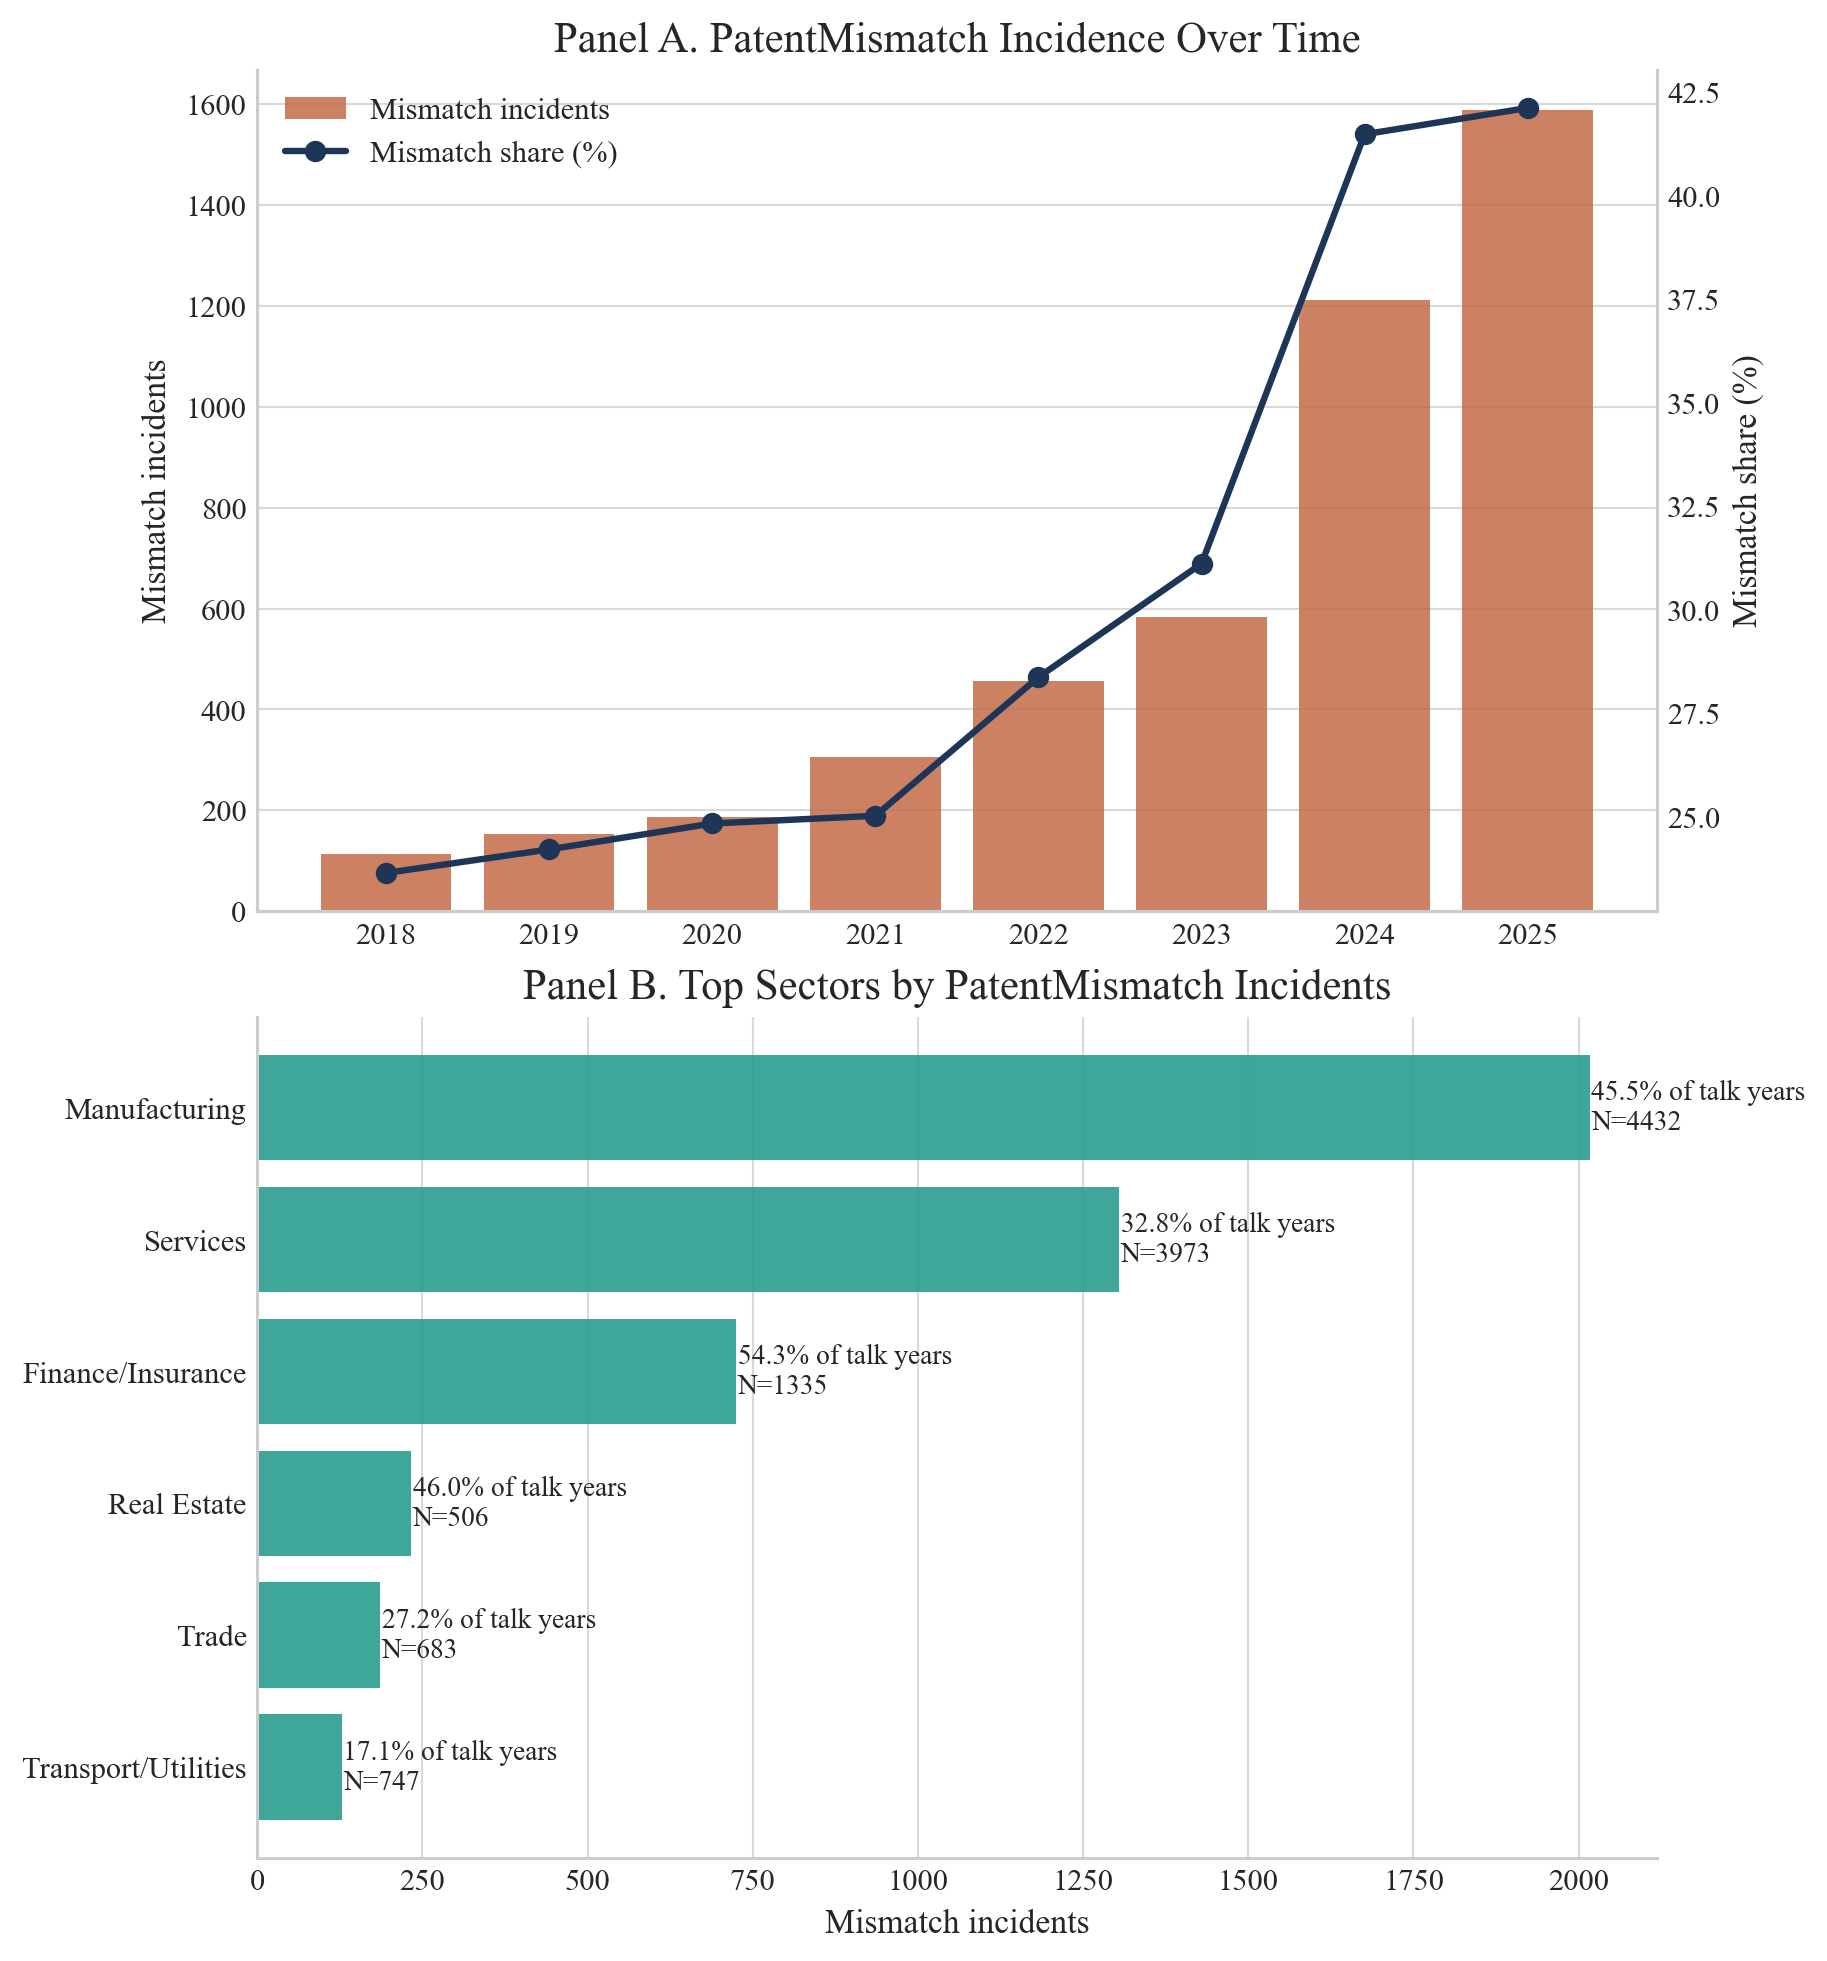
\includegraphics[width=\textwidth]{figures/figure1.png}
\caption{PatentMismatch surge through 2025}
\label{fig:mismatch_surge}
\end{figure}

Table~\ref{tab:summary_stats} describes the expanded ever-speaker annual panel and the linked filing-event sample used in the current paper. The panel contains 50,840 firm-year observations across 5,084 firms, of which 13,777 are AI-talking firm-years, and the classified corpus contains 147,879 AI-related sentences. AI-related disclosure remains highly skewed, and AI patenting remains sparse in the cross section, even within the ever-speaker universe. Those distributional features are important for interpretation. We are studying a setting in which narrative expansion has become widespread, while observable implementation remains concentrated in a much smaller subset of firms.

\tablepdf
{Summary statistics}
{tab:summary_stats}
{This table presents summary statistics for the variables used in the analysis. It reports the mean, standard deviation, selected percentiles, and the number of observations for the expanded ever-speaker annual panel.}
{tables/table1.png}

Figures~\ref{fig:descriptive_background} and \ref{fig:patent_background} provide a more general descriptive backdrop. Figure~\ref{fig:descriptive_background} traces the increase in the volume of AI-related disclosure and the evolution of disclosure composition over time. Figure~\ref{fig:patent_background} shows that AI patenting also increases over the sample, but much more gradually and at a lower base. With Figure~\ref{fig:mismatch_surge}, these descriptive patterns clarify why the mismatch construct is economically interesting. The growth in AI talk appears to outpace the growth in visible technological realization for a substantial subset of firms.

\begin{figure}[p]
\centering
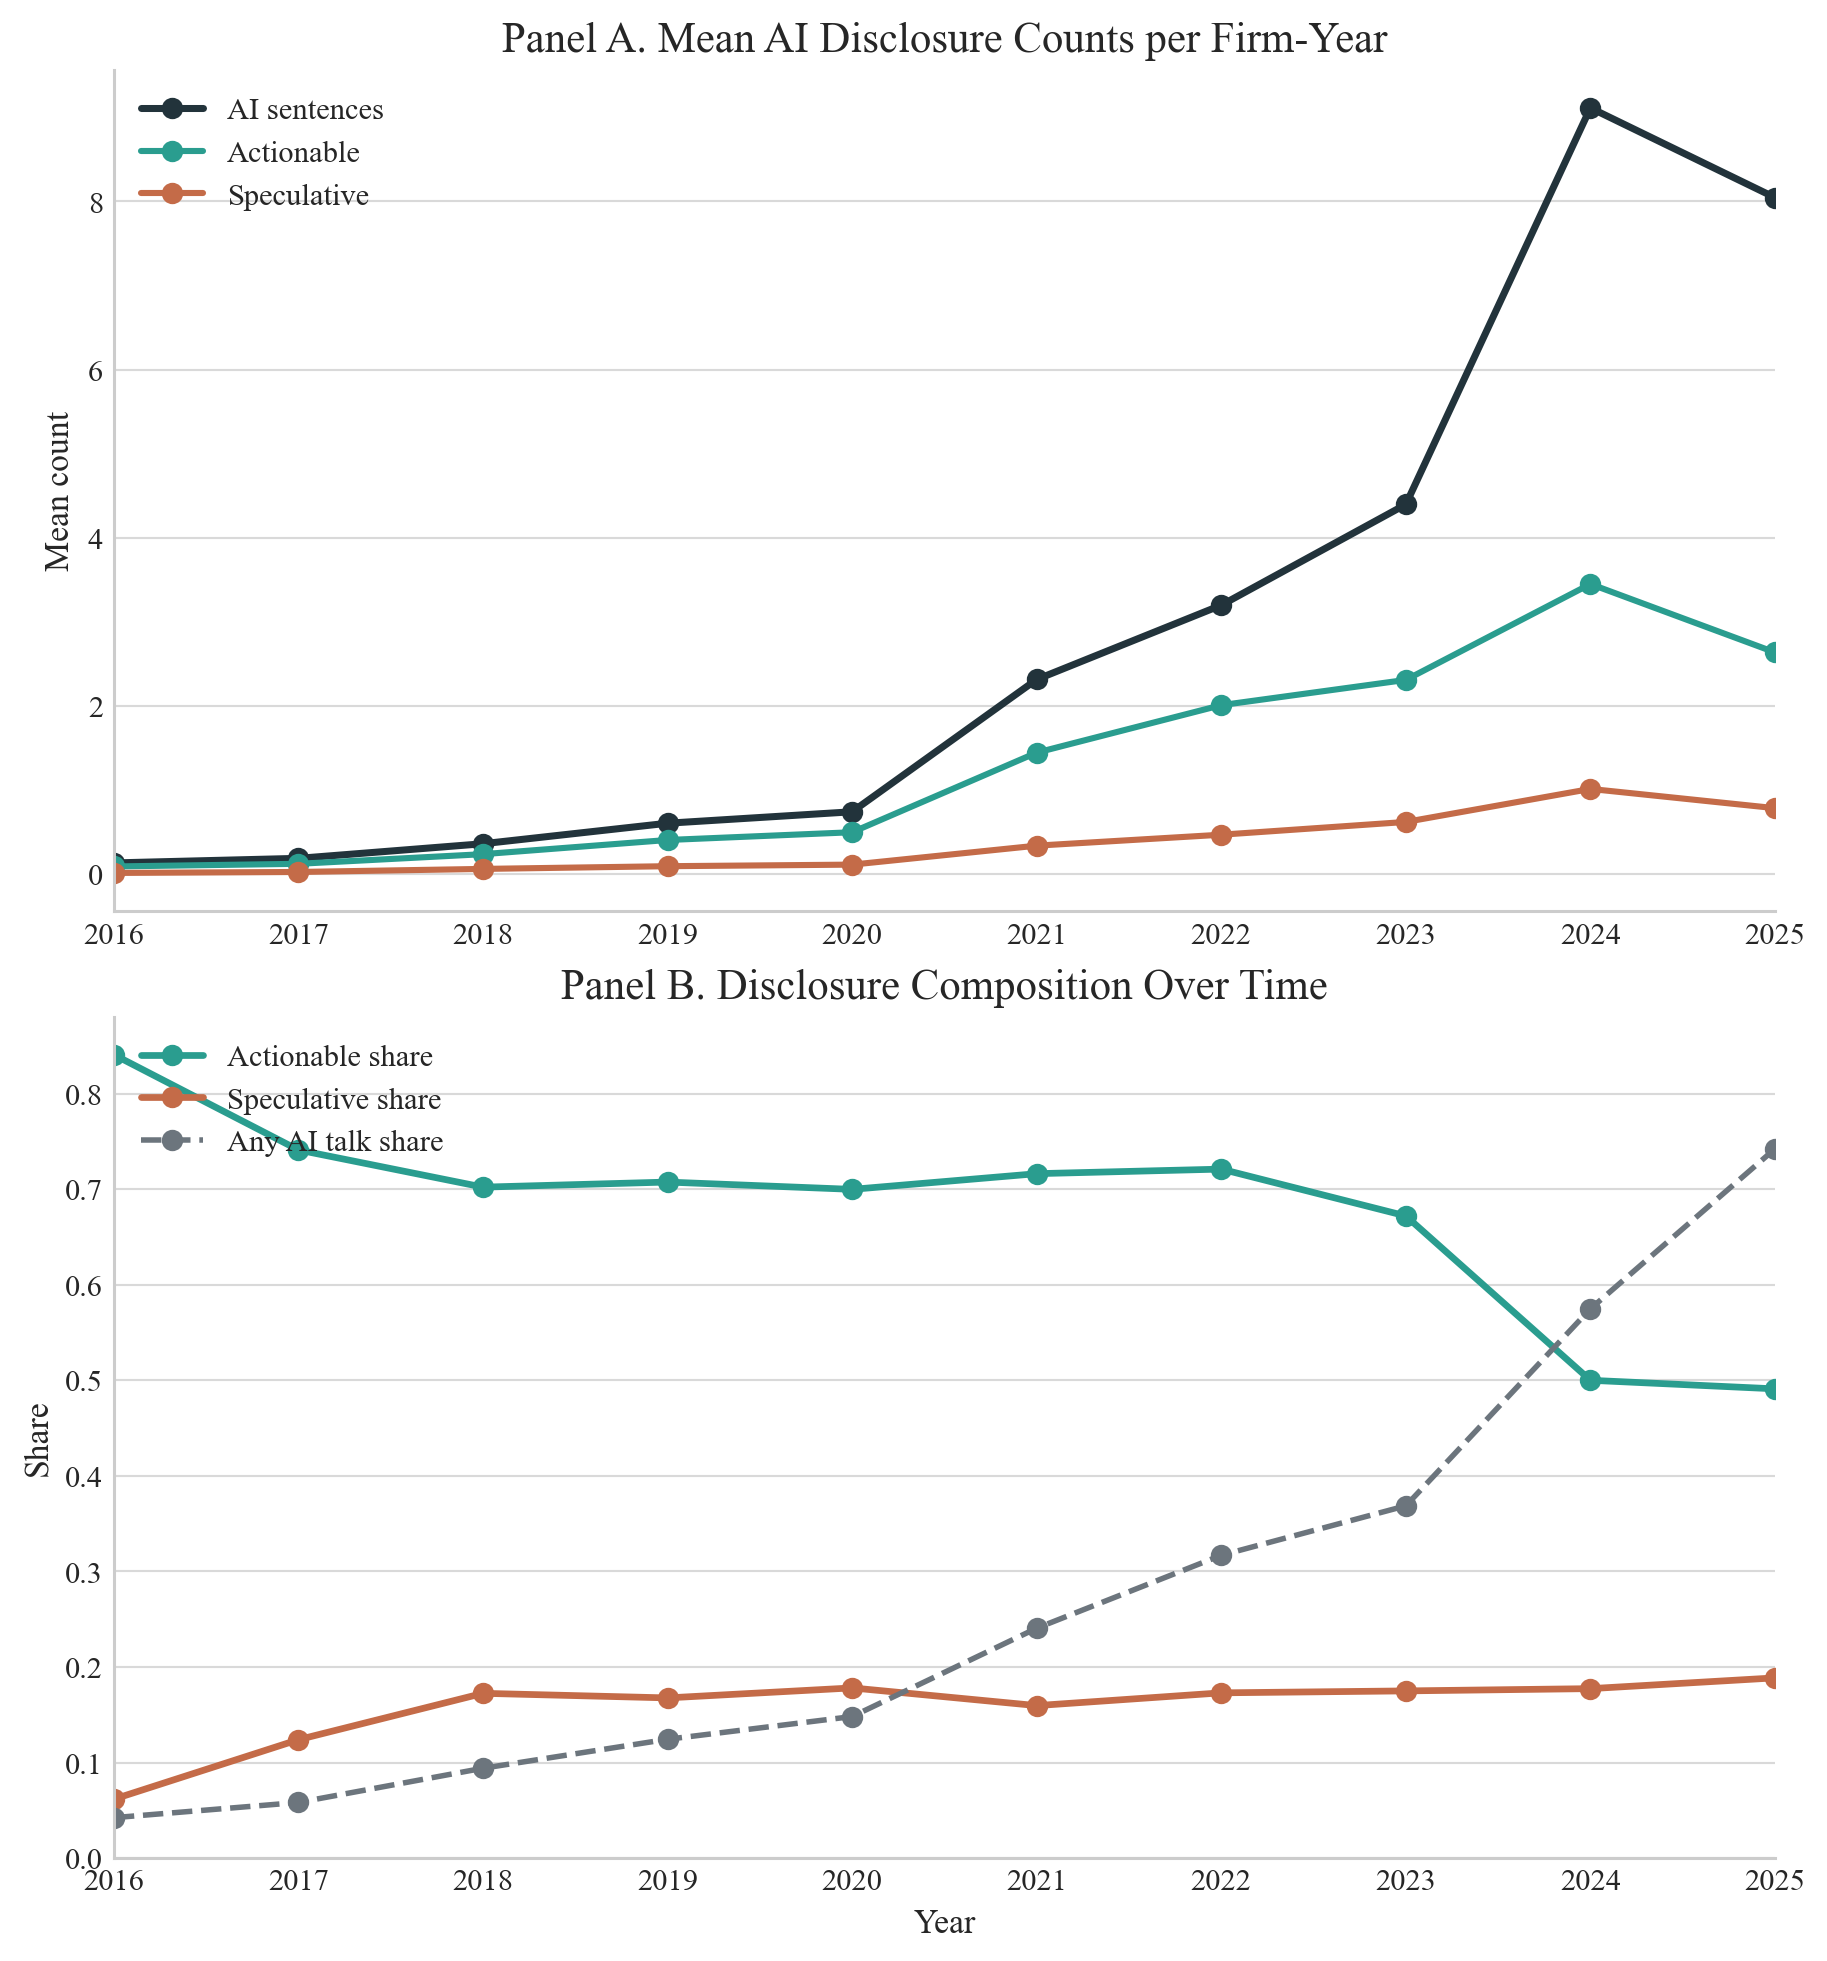
\includegraphics[width=\textwidth]{figures/figure2.png}
\caption{Disclosure volume and composition over time}
\label{fig:descriptive_background}
\end{figure}

\begin{figure}[p]
\centering
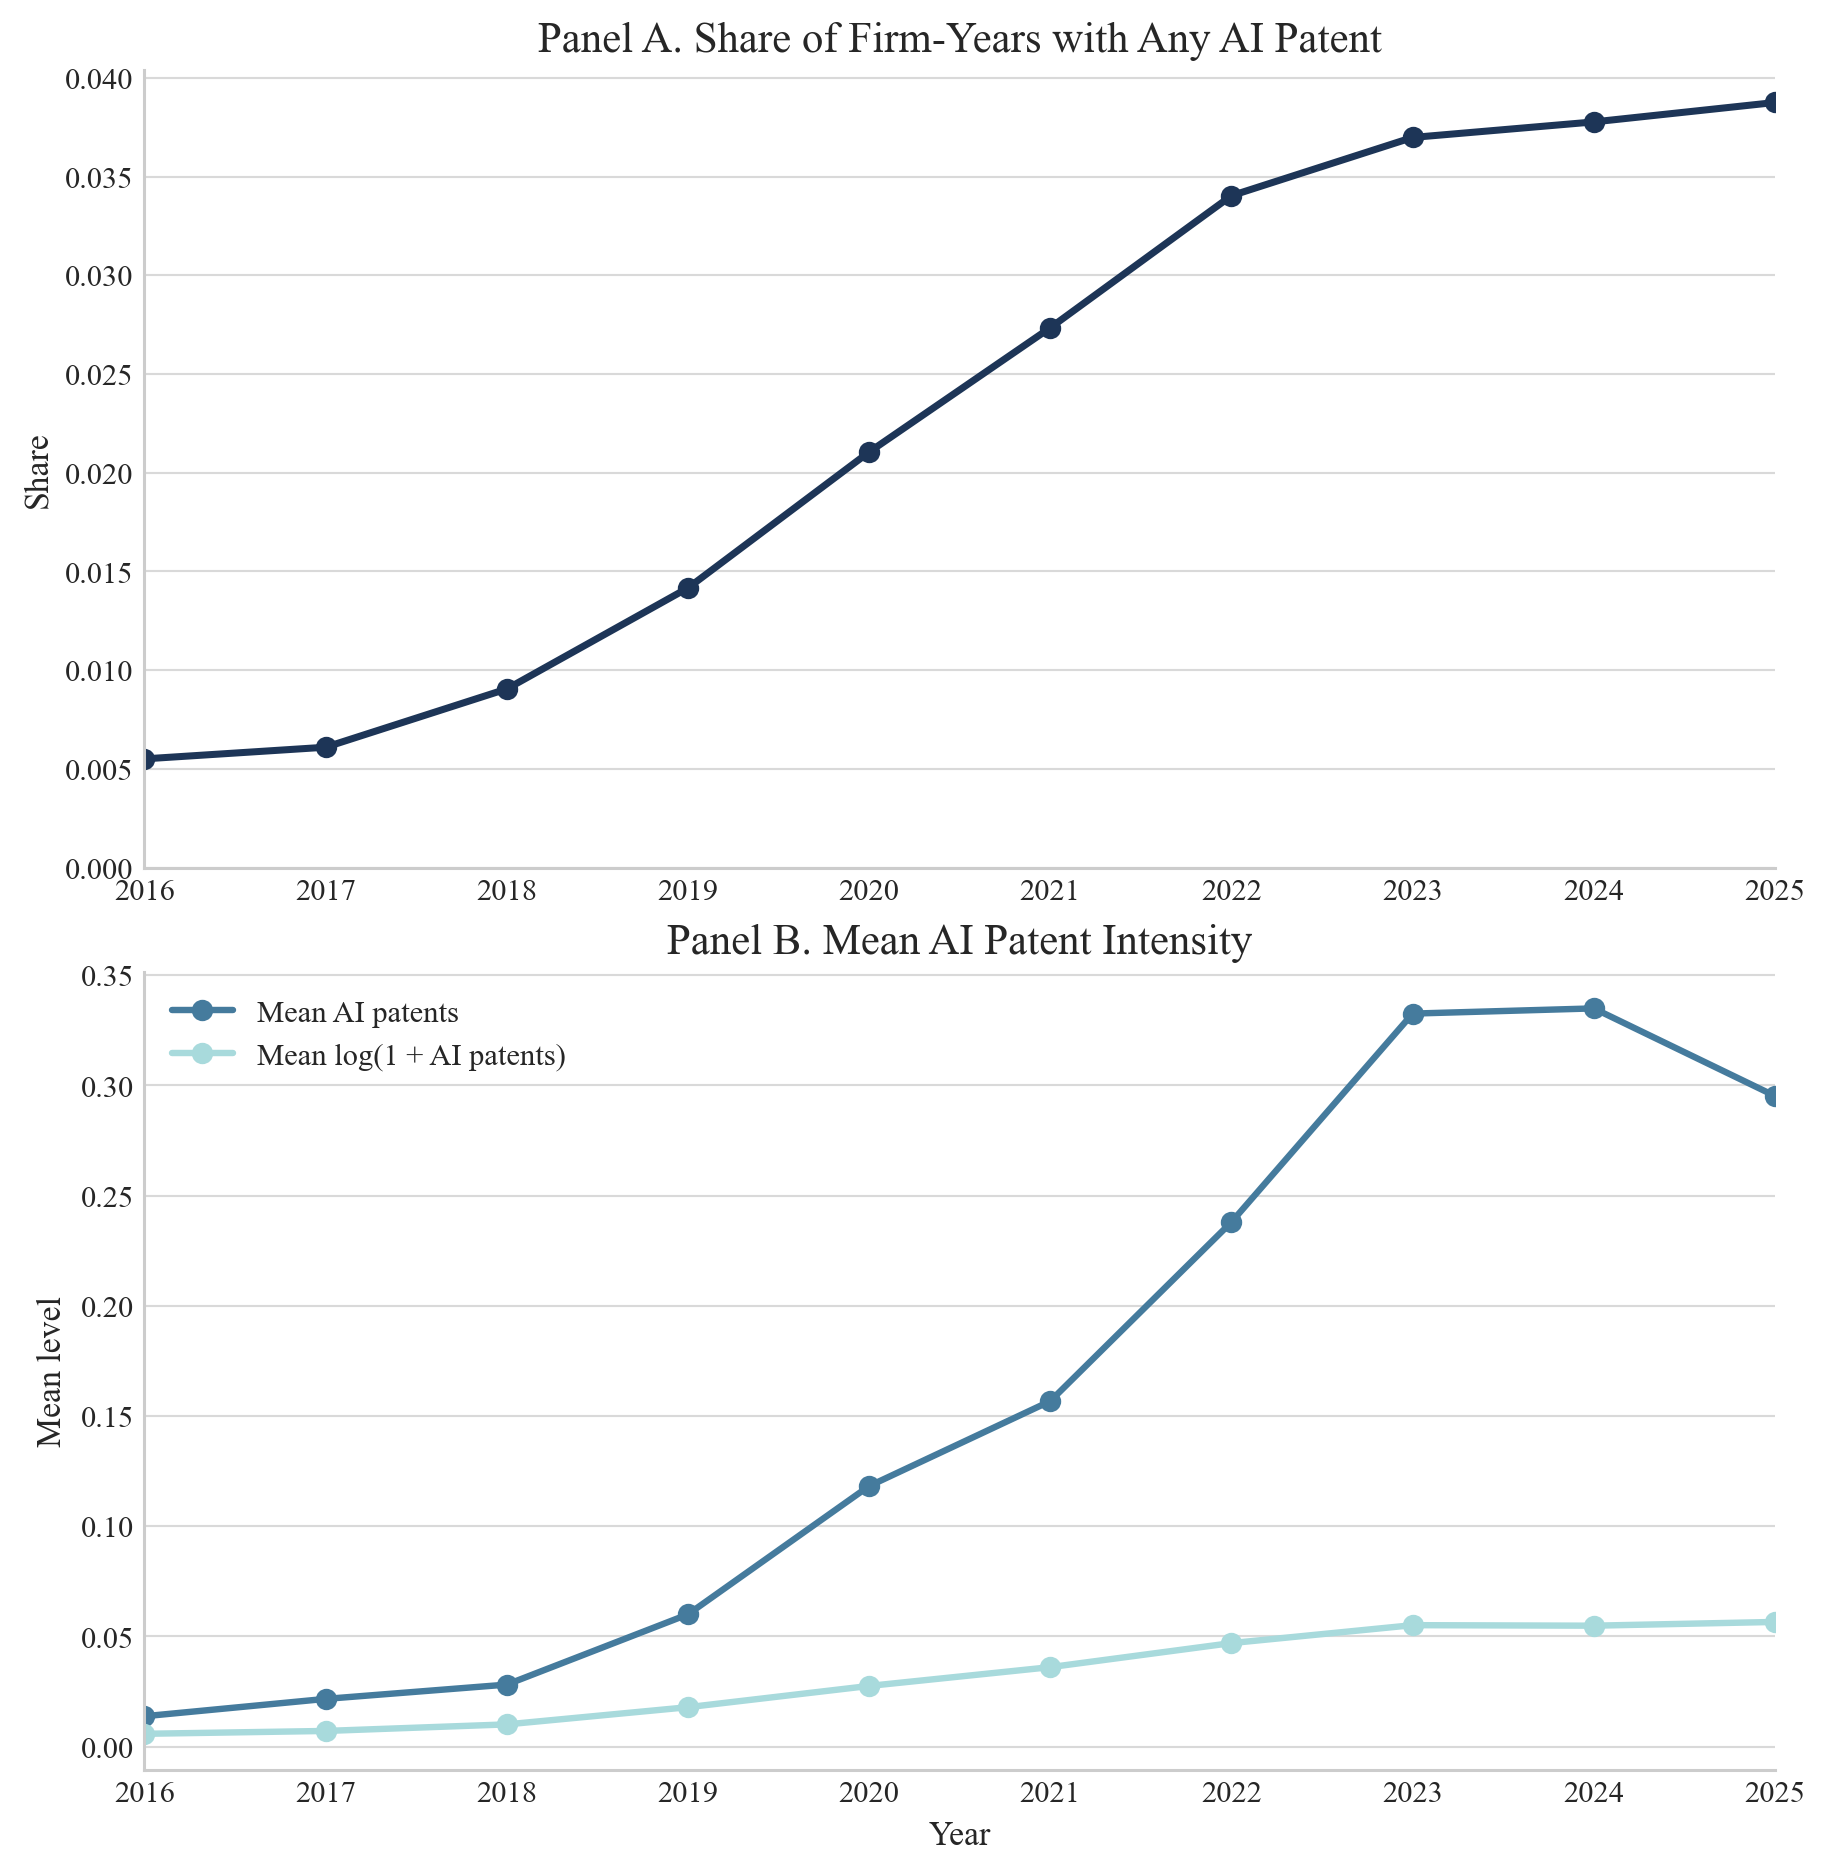
\includegraphics[width=\textwidth]{figures/figure3.png}
\caption{AI patent coverage over time}
\label{fig:patent_background}
\end{figure}

\subsection{Markets do not fully sort low-credibility AI disclosure at the filing date}

The first market-based question is whether investors distinguish low-credibility AI disclosure immediately when the annual 10-K is released. Table~\ref{tab:filing_date_car} suggests that they do not, at least not in a clean or robust way. In the narrow filing window, the difference in market-adjusted abnormal returns between mismatch and non-mismatch AI filers is small and statistically insignificant. The mismatch-minus-non-mismatch mean difference in CAR[$-1,+1$] is 0.115 percentage points with a p-value of 0.678, and the corresponding filing-level regression coefficient on PatentMismatch is 0.0015 with a p-value of 0.702. The same conclusion holds in the slightly wider CAR[$-2,+2$] window. The filing date does not appear to cleanly separate mismatch from non-mismatch firms in return space.

\tablepdf
{Filing-date abnormal returns around annual 10-K releases}
{tab:filing_date_car}
{This table reports market-adjusted filing-date cumulative abnormal returns around annual 10-K releases. Panel A reports mean CARs by PatentMismatch status and the mismatch-minus-non-mismatch difference. Panel B reports filing-level regressions of CAR on PatentMismatch, the AS ratio, and AI Focus with lagged controls, industry fixed effects, filing-year fixed effects, and standard errors clustered by firm. Statistical significance at the 1\%, 5\%, and 10\% levels is indicated by ***, **, and *, respectively. A CAR[$-5,+5$] column is not included in this first run because the current daily event-return scaffold starts at event day $-2$.}
{tables/table2.png}

\subsection{The sharper pricing pattern emerges after the filing}

If the filing date does not provide a clean correction, the next question is whether the pricing response unfolds more gradually. Figure~\ref{fig:post_filing_drift} and Table~\ref{tab:portfolio_alpha} suggest that it does. The event-time figure shows that the return paths separate after the filing window rather than at it, which is more consistent with slower incorporation than with an immediate market response. The sharper return-based pattern appears in the calendar-time portfolio tests. A long--short strategy that buys firms with more credible AI disclosure and shorts mismatch firms earns its strongest return over the subsequent quarter in the equal-weight specification. The equal-weight 3-month portfolio delivers a market alpha of 0.926 percentage points per month (p = 0.047), or approximately 11.2\% annualized. By contrast, the value-weighted 3-month alpha is essentially zero. The pattern weakens at the 12-month horizon. That combination of results suggests that the post-filing effect is concentrated in shorter horizons and outside the largest firms, which is consistent with a slower correction in harder-to-value companies rather than a broad market-wide repricing.

\begin{figure}[p]
\centering
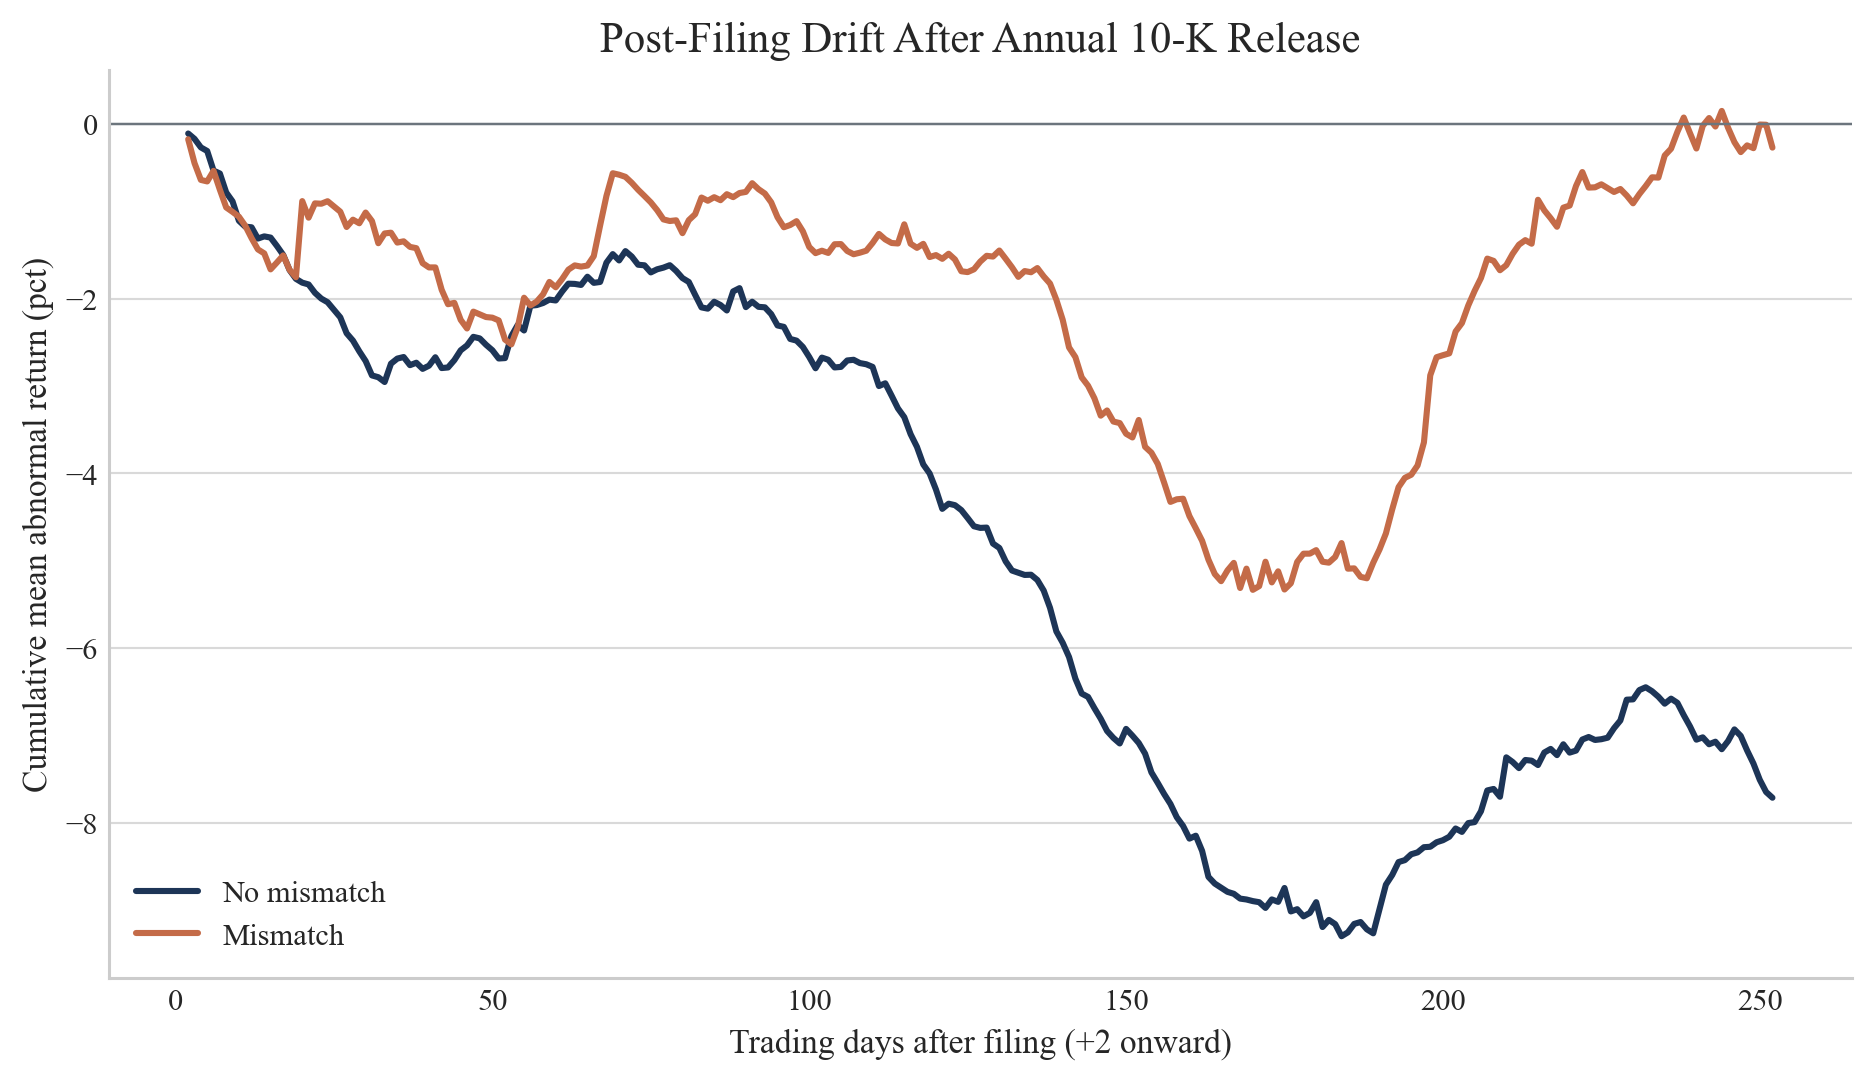
\includegraphics[width=\textwidth]{figures/figure4.png}
\caption{Post-filing drift after annual 10-K release}
\label{fig:post_filing_drift}
\end{figure}

\tablepdf
{Calendar-time long--short portfolio returns after filing signals}
{tab:portfolio_alpha}
{This table reports calendar-time long--short portfolio returns formed after AI-related annual filing signals. Each month, the long leg holds non-mismatch AI filers and the short leg holds mismatch AI filers that filed within the prior 1, 3, 6, or 12 months. Panel A reports equal-weight portfolios and Panel B reports value-weight portfolios using lagged market capitalization. Market alpha is the intercept from a regression of the long--short monthly return on the CRSP value-weighted market return. Panel C splits the three-month portfolio on whether the underlying filing signal occurred before or after the ChatGPT regime shift.}
{tables/table3.png}

\subsection{Cross-sectional valuation and financing consequences}

Valuation and financing tests ask whether the same disclosure-credibility construct appears in broader annual market outcomes. Table~\ref{tab:valuation_financing_nonbig} reports the cleaner non-big-firm specifications, where the current effects are strongest. The valuation results are positive and marginally significant: PatentMismatch is associated with higher log market-capitalization-to-assets and a higher log Tobin's-$Q$ proxy, with coefficients of 0.0619 (p = 0.065) and 0.0627 (p = 0.062), respectively. The financing side is much weaker. Neither next-year share growth nor the indicator for substantial issuance shows a meaningful relation to PatentMismatch in this sample. This implies that the more credible cross-sectional consequence in the current data is valuation, and that this valuation pattern is most visible outside the largest firms.

\tablepdf
{Financing and valuation consequences in non-big firms}
{tab:valuation_financing_nonbig}
{This table reports valuation and financing consequences associated with disclosure credibility in the non-big subsample. Panel A uses log market-capitalization-to-assets, a log Tobin's-$Q$ proxy equal to log(1 + market-capitalization-to-assets + leverage), and the next-year change in that log $Q$ proxy. Panel B uses next-year change in CRSP shares outstanding and an indicator for share growth above 5\%. The key regressors are PatentMismatch, the AS ratio, and AI Focus. All specifications absorb firm and year fixed effects and use firm-clustered standard errors.}
{tables/table4.png}

\subsection{Real consequences and validation of the disclosure construct}

Market-based evidence suggests that low-credibility AI disclosure is not fully sorted out at the filing date and that slower correction is strongest outside the largest firms. The next question is whether the same disclosure-credibility construct is informative for subsequent real outcomes. Table~\ref{tab:real_effects} reports that PatentMismatch is associated with materially lower future ROA at the two-year horizon, with a coefficient of $-0.0582$ (p = 0.004), while the AS ratio is negatively related to future sales growth at the one-year horizon, with a coefficient of $-0.0826$ (p = 0.009), suggesting that the disclosure-credibility construct has a forward link to operating and innovation-related outcomes beyond the immediate market-response block.

\tablepdf
{Real effects beyond immediate market outcomes}
{tab:real_effects}
{This table reports forward operating and innovation-related outcomes associated with disclosure credibility. The dependent variables include future ROA and future sales growth at annual horizons. The key regressors are PatentMismatch, the AS ratio, and AI Focus. All specifications use the annual ever-speaker panel and absorb firm and year fixed effects with firm-clustered standard errors.}
{tables/table5.png}

The next question is whether the disclosure composition itself still behaves as expected once  beyond broad AI-talk counts. Table~\ref{tab:composition_timing} reports that actionable disclosure remains positively associated with later AI-related patenting, with coefficients of 0.042 in both $t$ and $t+1$, and 0.039 in $t+2$, which are all strongly significant. Speculative-only disclosure behaves differently. Its coefficient is negative at $t$ ($-0.044$, p $< 0.05$) and effectively disappears by $t+1$. The market and mismatch analysis therefore rest on a disclosure measure that continues to separate more implementation-linked AI language from weaker, more rhetorical AI language.

\tablepdf
{Disclosure composition and AI patent timing}
{tab:composition_timing}
{This table reports annual panel regressions linking disclosure composition to AI patent timing. Panel A uses the actionable-disclosure indicator and Panel B uses the speculative-only indicator. The dependent variable is $\log(1+\text{AI patents})$ evaluated at horizons from $t-2$ through $t+2$. All columns include the baseline annual control set together with firm and year fixed effects and firm-clustered standard errors.}
{tables/table6.png}

Table~\ref{tab:mismatch_tplus1} then returns to the core validation test. The specification focuses on the AS ratio and its interaction with PatentMismatch, using future AI patenting at $t+1$ as the outcome. In the firm-plus-year fixed-effects column, the AS ratio enters positively at 0.038 (p $< 0.01$), while the interaction with PatentMismatch enters negatively at $-0.078$ (p $< 0.01$). Among non-mismatch firm-years, a higher AS ratio is associated with stronger subsequent AI patenting. In mismatch firm-years, that relation is materially weaker. This is the clearest evidence that the same disclosure-composition signal maps differently to later innovation depending on whether contemporaneous patent weakness is already present.

\tablepdf
{AS ratio, PatentMismatch, and future AI patenting at $t+1$}
{tab:mismatch_tplus1}
{This table reports the main construct-validation specification. The dependent variable is $\log(1+\text{AI patents})$ at $t+1$. The key regressors are the AS ratio and its interaction with PatentMismatch. Columns vary the fixed-effects structure and sample trim while holding the annual control set fixed. Standard errors are clustered at the firm level.}
{tables/table7.png}

Figure~\ref{fig:mismatch_alignment} traces the fitted relation between the AS ratio and future AI patenting separately for mismatch and non-mismatch firm-years. In non-mismatch observations, higher AS-ratio bins are associated with stronger subsequent AI patenting. In mismatch observations, the relation is substantially flatter and in some ranges turns negative. The figure makes the interaction result in Table~\ref{tab:mismatch_tplus1} visible: the same disclosure-composition signal has a much weaker innovation content in the subset of firm-years already flagged as low credibility.

\begin{figure}[p]
\centering
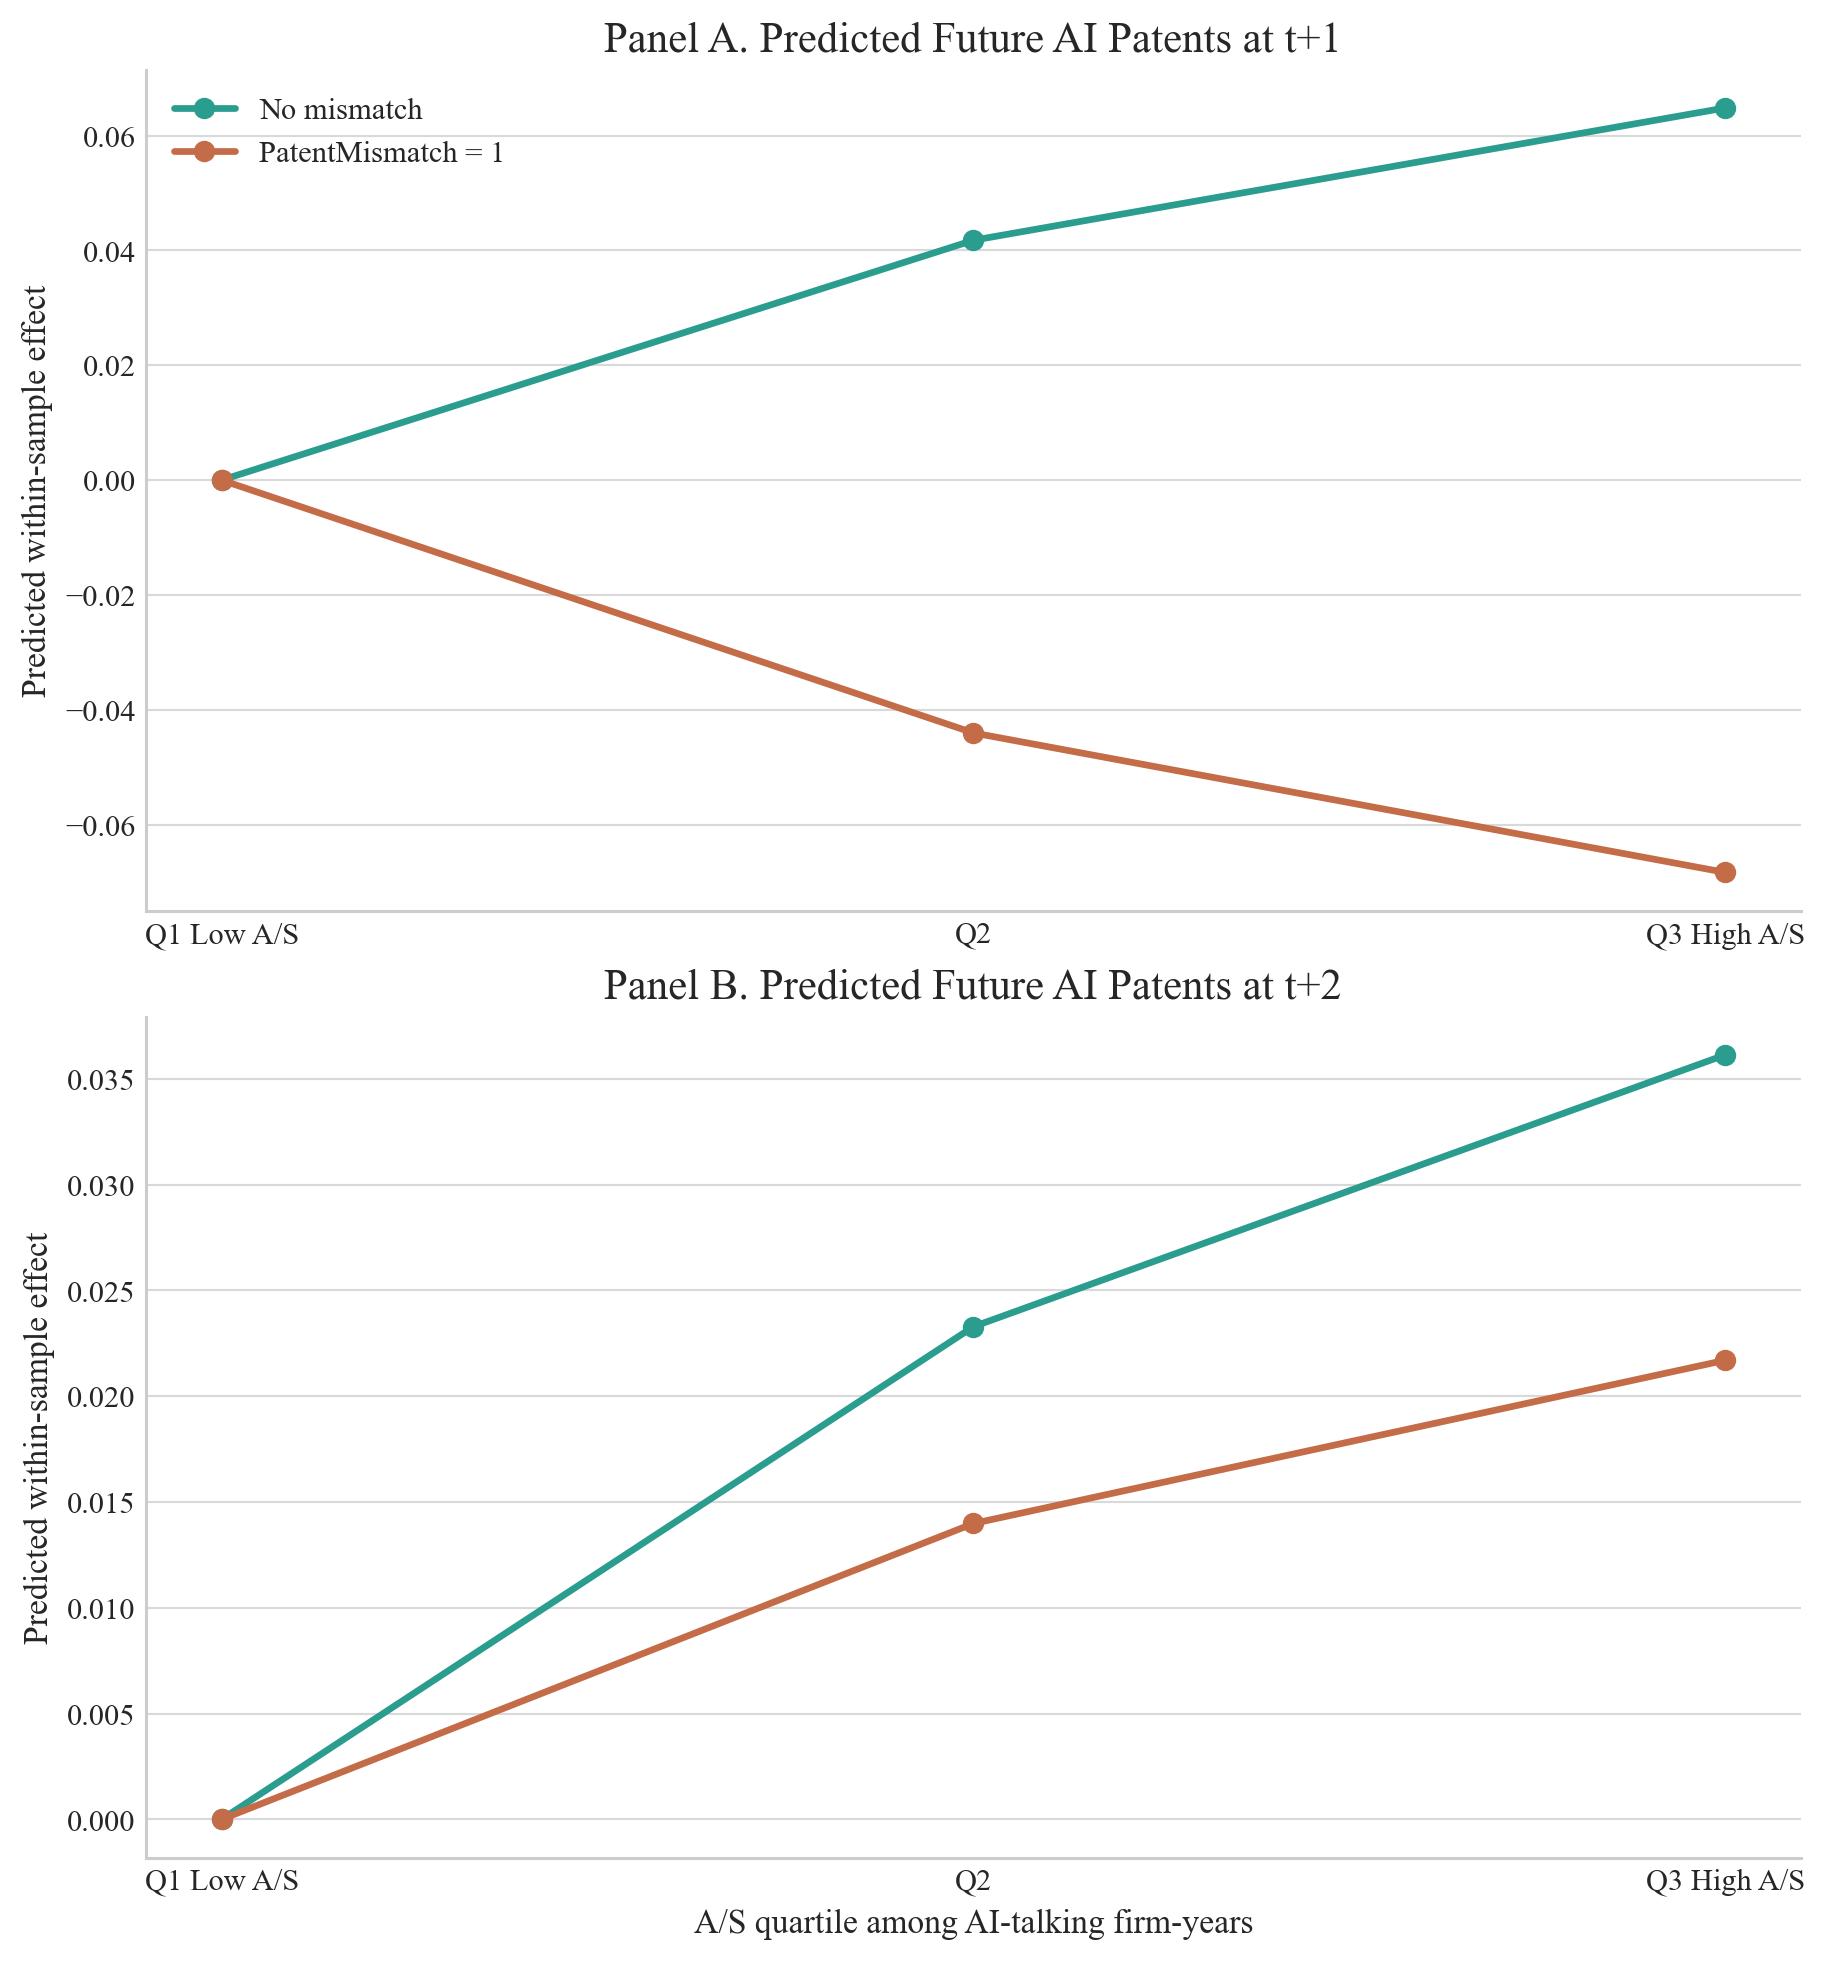
\includegraphics[width=\textwidth]{figures/figure5.png}
\caption{Patent alignment and mismatch by AS-ratio quantile}
\label{fig:mismatch_alignment}
\end{figure}

\subsection{Exploratory evidence around the release of ChatGPT}

The final question is whether the disclosure-credibility patterns intensify after the public release of ChatGPT. Table~\ref{tab:chatgpt_did} reports the baseline post-ChatGPT difference-in-differences specifications, where treated firms are those with weak pre-period AI capability, firms with zero pre-period AI-related patents, and either a low pre-period AS ratio or no pre-period actionable disclosure. The strongest response appears in PatentMismatch: the post-ChatGPT interaction is 0.1745 (p $<$ 0.001). By contrast, the CAR filing-date interaction is 0.0076 (p = 0.307), and the post-filing BHAR interaction is 0.0075 (p = 0.737). In other words, the post-ChatGPT evidence is most consistent with an expansion in low-credibility AI talk rather than with a comparably sharp immediate repricing of that talk by the market.

These results should be interpreted cautiously. The PatentMismatch panel shows a strong post-2022 response, whereas the corresponding CAR panel does not. The pretrend diagnostics are also less comfortable for PatentMismatch than for CAR. For that reason, the post-ChatGPT block is best viewed as exploratory evidence that the late-2022 period amplified the disclosure-credibility tension documented elsewhere in the paper.

\tablepdf
{Exploratory post-ChatGPT difference-in-differences evidence}
{tab:chatgpt_did}
{The table reports exploratory post-ChatGPT difference-in-differences evidence on whether the post-2022 period is associated with a sharper expansion in low-credibility AI disclosure.}
{tables/table8.png}
\FloatBarrier

The appendix collects the supporting material that is useful for interpretation but not essential to the main narrative. Appendix A reports the updated measurement audit and the sample-attrition map. Appendix B reports the broader patent-timing validation tables and the longer-horizon mismatch specification. Appendix C reports the determinants, heterogeneity, and ancillary consequence tests, including the fuller post-ChatGPT event-study figure.

\section{Conclusion}
We study whether markets and later innovation outcomes distinguish between more credible and less credible AI disclosure in annual 10-K filings. Using U.S. public firms from 2016 to 2025, we classify AI-related sentences as actionable, speculative, or irrelevant, aggregate those classifications into firm-year disclosure measures, and use them to construct the AS ratio and PatentMismatch. Results show that low-credibility AI disclosure becomes common quickly in the post-2022 period: PatentMismatch characterizes 41.5\% of AI-talking firm-years in 2024 and 42.1\% in 2025. That pattern is difficult to reconcile with a view in which the recent expansion of AI language in corporate filings simply mirrors a comparable expansion in verifiable technological implementation.

The market evidence indicates that this divergence is not fully resolved at the filing date. Filing-date abnormal returns show little clean evidence of immediate discipline, whereas the stronger correction appears after disclosure. A long--short strategy that buys firms with more credible AI disclosure and shorts mismatch firms earns its strongest return over the subsequent quarter, with an equal-weight alpha of 0.93\% per month, or roughly 11.2\% annualized. The corresponding value-weight result is much weaker, Suggesting that the slower correction is concentrated outside the largest firms. Cross-sectional valuation evidence points in the same direction. At the same time, the disclosure construct remains anchored to later technological realization: actionable AI language aligns more closely with subsequent AI patenting than speculative language, and the AS-ratio $\times$ PatentMismatch specification predicts weaker future AI patent output. Exploratory post-ChatGPT tests are directionally consistent with this interpretation, although they are better understood as suggestive rather than as the primary identification strategy.

The contribution lies in the combination of these results with the underlying measurement design. Prior work has shown that AI-related language in corporate disclosure is informative and that markets react to AI narratives, while recent studies have begun to distinguish AI talk from AI walk more directly. The present paper contributes by centering mandatory annual filings, scaling the actionable-versus-speculative distinction into a reusable audited framework, and introducing PatentMismatch as a filing-based construct that combines disclosure composition with contemporaneous patent weakness. This makes it possible to study low-credibility AI disclosure in a way that is portable across samples and informative both for later innovation outcomes and for market consequences.

Several limitations remain. Because PatentMismatch firms may differ systematically from non-mismatch firms along observable and unobservable dimensions, the return-based evidence is best interpreted as consistent with slower incorporation of disclosure credibility rather than as definitive proof that the pricing differential is caused solely by AI-washing. The post-ChatGPT tests should likewise be understood as exploratory rather than decisive. Some of the market-based patterns are also materially stronger outside the largest firms, which suggests that mispricing and disclosure credibility may be most relevant in settings where valuation is harder and external verification is weaker. The evidence suggests that low-credibility AI disclosure is economically important not only because it departs from later technological realization, but also because markets do not appear to fully price that gap immediately. More broadly, the results point to a setting in which the cost of AI talk can fall more quickly than the cost of real AI implementation, and in which disclosure composition provides a useful way to distinguish the two.

\appendix

\renewcommand{\thesection}{Appendix \Alph{section}}
\counterwithin*{table}{section}
\renewcommand{\thetable}{\Alph{section}\arabic{table}}
\counterwithin*{figure}{section}
\renewcommand{\thefigure}{\Alph{section}\arabic{figure}}

\clearpage
\section{Measurement audit and sample construction diagnostics}
This appendix reports the measurement audit and sample-construction diagnostics referenced in Sections~3.1 and 3.2.

\apptablepdf
{Measurement audit of the AI-disclosure classification pipeline}
{tab:appendix_audit}
{This table reports the updated measurement audit for the disclosure-classification layer. Panel A summarizes the adjudicated sentence base, the leakage-safe training and calibration pool, the heldout-v4 benchmark, and the human--human IRR rerun. Panel B reports heldout-v4 evaluation metrics for the selected hybrid classifier.}
{tables/tableA1.png}

\apptablepdf
{Sample attrition map across empirical blocks}
{tab:appendix_attrition}
{This table maps sample changes across the main empirical blocks. The differences in sample size are mechanical consequences of the annual timing design, complete-case control requirements, CRSP availability in event windows, and the shift from firm-year panels to the 2016 firm-level cross-section in the determinants appendix.}
{tables/tableA2.png}

\apptablepdf
{Classifier-risk robustness: high-confidence composition tests}
{tab:appendix_highconf_comp}
{This table reports composition-based robustness checks using high-confidence sentence classifications only. The purpose is to assess whether the main directional patterns strengthen when the disclosure measures are restricted to the most confidently classified sentences.}
{tables/tableA3.png}

\apptablepdf
{Classifier-risk robustness: high-confidence mismatch tests}
{tab:appendix_highconf_mismatch}
{This table reports mismatch-based robustness checks using high-confidence sentence classifications only. The purpose is to assess whether the main PatentMismatch patterns remain when the disclosure layer is restricted to the most confidently classified sentences.}
{tables/tableA4.png}

\apptablepdf
{Variable definitions}
{tab:appendix_var_defs}
{This table defines the main disclosure, patent, event-study, valuation, financing, and control variables used in the analysis. Canonical field names are included so that the paper-facing labels map directly to the underlying panel construction and publication-run outputs.}
{tables/tableA5.png}

\clearpage
\section{Supplementary validation and patent-timing results}
This appendix reports supplementary validation and patent-timing results that support the main disclosure-credibility design.

\apptablepdf
{AI disclosure intensity and AI patent timing}
{tab:appendix_aifocus_timing}
{This table presents annual panel regressions relating broad AI disclosure intensity to AI patent timing at horizons from $t-2$ through $t+2$. It provides the broad-intensity validation backbone that complements the composition-based evidence emphasized in the main text.}
{tables/tableB1.png}

\apptablepdf
{Actionable disclosure and AI patent timing}
{tab:appendix_actionable_timing}
{This table presents the distributed-lag style timing matrix for actionable disclosure, relating the actionable-disclosure indicator to AI patent timing from $t-2$ through $t+2$.}
{tables/tableB2.png}

\apptablepdf
{Speculative-only disclosure and AI patent timing}
{tab:appendix_speculative_timing}
{This table presents the distributed-lag style timing matrix for speculative-only disclosure, relating the speculative-only indicator to AI patent timing from $t-2$ through $t+2$.}
{tables/tableB3.png}

\apptablepdf
{AS ratio, PatentMismatch, and longer-horizon AI patenting}
{tab:appendix_mismatch_tplus2}
{This companion table reports the longer-horizon version of the AS-ratio $\times$ PatentMismatch design using $\log(1+\text{AI patents})$ at $t+2$ as the outcome.}
{tables/tableB4.png}

\clearpage
\section{Determinants, heterogeneity, and ancillary consequence tests}
This appendix reports supplementary determinants, heterogeneity, and ancillary consequence tests referenced in the main text.

\apptablepdf
{Reduced-baseline determinants of PatentMismatch}
{tab:appendix_det_reduced}
{This table revisits the firm-level PatentMismatch determinants specification using the reduced baseline characteristic set. The dependent variable is an indicator for whether the firm records at least one PatentMismatch incident during 2016--2025. Baseline characteristics are measured in 2016 and include log assets, cash/assets, leverage, CAPX/assets, and ROA. This reduced specification preserves sample size relative to the fuller baseline set.}
{tables/tableC1.png}

\apptablepdf
{Full-baseline determinants of PatentMismatch}
{tab:appendix_det_full}
{This table presents the fuller cross-sectional determinants specification for whether a firm records at least one PatentMismatch incident during 2016--2025. Baseline characteristics are measured in 2016 and include log assets, cash/assets, leverage, R\&D/assets, CAPX/assets, ROA, and employees.}
{tables/tableC2.png}

\apptablepdf
{Full-baseline determinants of PatentMismatch intensity}
{tab:appendix_det_intensity}
{This companion table uses the share of AI-talking years flagged as PatentMismatch during 2016--2025 as the dependent variable rather than the extensive-margin indicator. The baseline characteristics are measured in 2016 and correspond to the full baseline set.}
{tables/tableC3.png}

\apptablepdf
{Small-firm heterogeneity in AI-washing pricing effects}
{tab:appendix_size_heterogeneity}
{This table reports heterogeneity in the filing-date and post-filing pricing effects by firm size. Small firms are defined using the monthly active-sample median lagged market capitalization from CRSP. The table is included as supporting evidence because the cleaner return and valuation patterns in the current draft are concentrated outside the largest firms.}
{tables/tableC4.png}

\begin{figure}[p]
\centering
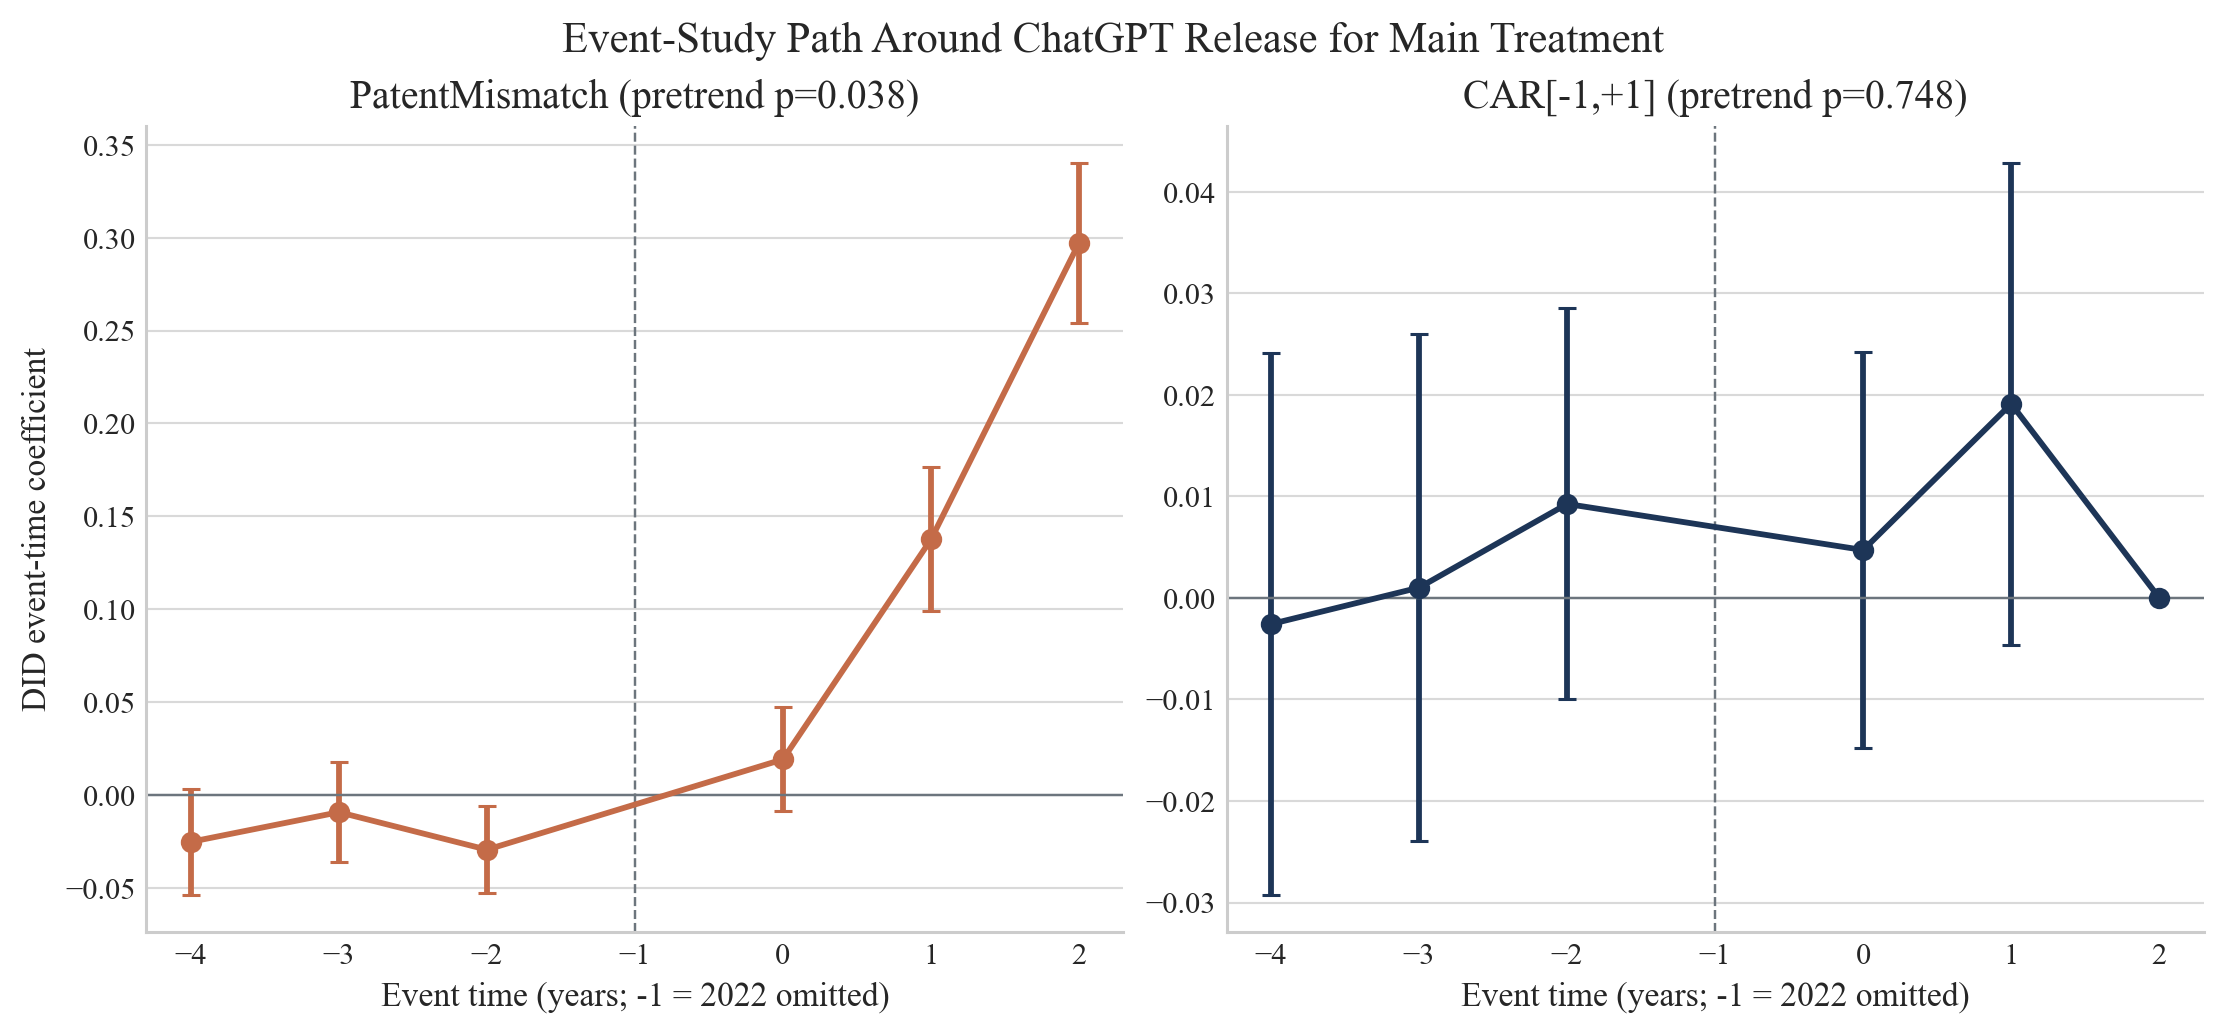
\includegraphics[width=\textwidth]{figures/figureC1.png}
\caption{Event-study path around the release of ChatGPT}
\label{fig:appendix_chatgpt_eventstudy}
\caption*{\footnotesize This figure plots the event-time coefficients for the baseline post-ChatGPT treatment around late 2022. The left panel reports PatentMismatch and the right panel reports filing-date CAR[$-1,+1$]. The figure is included as supporting evidence because the PatentMismatch response is visually strong after the break, but the pretrend diagnostics are not clean enough for this design to carry the paper's central identification burden.}
\end{figure}

\clearpage
\clearpage
\section*{References}

\begingroup
\small
\raggedright
\setlength{\parindent}{0pt}
\setlength{\parskip}{0.6em}
\emergencystretch=3em
\urlstyle{same}
\sloppy

Babina, T., Fedyk, A., He, A., \& Hodson, J. (2024). Artificial intelligence, firm growth, and product innovation. \textit{Journal of Financial Economics, 151}, 103745. \url{https://doi.org/10.1016/j.jfineco.2023.103745}

Baker, A. C., Larcker, D. F., McClure, C. G., Saraph, D., \& Watts, E. M. (2024). Diversity washing. \textit{Journal of Accounting Research, 62}(5), 1661--1709. \url{https://doi.org/10.1111/1475-679X.12542}

Bandyopadhyay, A. P., Mai, D., \& Pukthuanthong, K. (2023). AI narrative and stock mispricing. Working paper. \url{https://ssrn.com/abstract=4418236}

Barber, B. M., \& Odean, T. (2008). All that glitters: The effect of attention and news on the buying behavior of individual and institutional investors. \textit{The Review of Financial Studies, 21}(2), 785--818. \url{https://doi.org/10.1093/rfs/hhm079}

Barrios, J., Campbell, J., Johnson, R., \& Liu, Y. (2025). Artificially intelligent or artificially inflated? Determinants and informativeness of corporate AI disclosures. \textit{SSRN Electronic Journal}. \url{https://doi.org/10.2139/ssrn.5133107}

Basnet, A., Elias, M., Salganik-Shoshan, G., Walker, T., \& Zhao, Y. (2025). Analyzing the market’s reaction to AI narratives in corporate filings. \textit{International Review of Financial Analysis, 105}, 104378. \url{https://doi.org/10.1016/j.irfa.2025.104378}

Bellstam, G., Bhagat, S., \& Cookson, J. A. (2021). A text-based analysis of corporate innovation. \textit{Management Science, 67}(7), 4004--4031. \url{https://doi.org/10.1287/mnsc.2020.3682}

Beyer, A., Cohen, D. A., Lys, T. Z., \& Walther, B. R. (2010). The financial reporting environment: Review of the recent literature. \textit{Journal of Accounting and Economics, 50}(2), 296--343. \url{https://doi.org/10.1016/j.jacceco.2010.10.003}

Cao, S., Jiang, W., Yang, B., \& Zhang, A. L. (2023). How to talk when a machine is listening: Corporate disclosure in the age of AI. \textit{The Review of Financial Studies, 36}(9), 3603--3642. \url{https://doi.org/10.1093/rfs/hhad021}

Cao, Y., Liu, M., Qiu, J., \& Zhao, R. (2024). Information in disclosing emerging technologies: Evidence from AI disclosure (SSRN Scholarly Paper No. 4987085). \textit{Social Science Research Network}. \url{https://doi.org/10.2139/ssrn.4987085}

Cohen, L., Malloy, C., \& Nguyen, Q. (2020). Lazy Prices. \textit{The Journal of Finance, 75(3)}, 1371–1415. \url{https://doi.org/10.1111/jofi.12885}

Crawford, V. P., \& Sobel, J. (1982). Strategic information transmission. \textit{Econometrica, 50}(6), 1431--1451. \url{https://doi.org/10.2307/1913390}

Davis, A. K., Piger, J. M., \& Sedor, L. M. (2012). Beyond the numbers: Measuring the information content of earnings press release language. \textit{Contemporary Accounting Research, 29}(3), 845--868. \url{https://doi.org/10.1111/j.1911-3846.2011.01130.x}

Delmas, M. A., \& Burbano, V. C. (2011). The drivers of greenwashing. \textit{California Management Review, 54}(1), 64--87. \url{https://doi.org/10.1525/cmr.2011.54.1.64}

Donelson, D., Kim, M., Kim, S., \& Yip, M. (2025). Strategic AI disclosures: Determinants and consequences of obfuscated and overstated AI investments. \textit{SSRN Electronic Journal}. \url{https://doi.org/10.2139/ssrn.5265257}

Dye, R. A. (1985). Disclosure of nonproprietary information. \textit{Journal of Accounting Research, 23}(1), 123--145. \url{https://doi.org/10.2307/2490910}

Fu, X., Wu, X., \& Zhang, Z. (2021). The information role of earnings conference call tone: Evidence from stock price crash risk. \textit{Journal of Business Ethics, 173}(3), 643--660. \url{https://doi.org/10.1007/s10551-019-04326-1}

Gigler, F. (1994). Self-enforcing voluntary disclosures. \textit{Journal of Accounting Research, 32}(2), 224--240. \url{https://doi.org/10.2307/2491283}

Grossman, S. J. (1981). The informational role of warranties and private disclosure about product quality. \textit{The Journal of Law and Economics, 24}(3), 461--483. \url{https://doi.org/10.1086/466995}

Healy, P. M., \& Palepu, K. G. (2001). Information asymmetry, corporate disclosure, and the capital markets: A review of the empirical disclosure literature. \textit{Journal of Accounting and Economics, 31}(1), 405--440. \url{https://doi.org/10.1016/S0165-4101(01)00018-0}

Huang, X., Teoh, S. H., \& Zhang, Y. (2014). Tone management. \textit{The Accounting Review, 89}(3), 1083--1113. \url{https://doi.org/10.2308/accr-50684}

Hummel, K., \& Schlick, C. (2016). The relationship between sustainability performance and sustainability disclosure -- Reconciling voluntary disclosure theory and legitimacy theory. \textit{Journal of Accounting and Public Policy, 35}(5), 455--476. \url{https://doi.org/10.1016/j.jaccpubpol.2016.06.001}

Jia, N., Li, N., Ma, G., \& Xu, D. (2025). Corporate responses to generative AI: Early evidence from conference calls. \textit{Review of Accounting Studies}. \url{https://doi.org/10.1007/s11142-025-09916-1}

Kim, E.-H., \& Lyon, T. P. (2015). Greenwash vs. brownwash: Exaggeration and undue modesty in corporate sustainability disclosure. \textit{Organization Science, 26}(3), 705--723. \url{https://doi.org/10.1287/orsc.2014.0949}

Kim, J., \& Valentine, K. (2023). Public firm disclosures and the market for innovation. \textit{Journal of Accounting and Economics, 76}(1), 101577. \url{https://doi.org/10.1016/j.jacceco.2023.101577}

Li, B. (2026). AI washing. Working paper.

Li, F. (2010). The information content of forward-looking statements in corporate filings -- A naïve Bayesian machine learning approach. \textit{Journal of Accounting Research, 48}(5), 1049--1102. \url{https://doi.org/10.1111/j.1475-679X.2010.00382.x}

Liu, J. (2023). AI exposure without labor data: Measuring AI’s impact through firms (SSRN Scholarly Paper No. 4668083). \textit{Social Science Research Network}. \url{https://doi.org/10.2139/ssrn.4668083}

Loughran, T., \& McDonald, B. (2011). When is a liability not a liability? Textual analysis, dictionaries, and 10-Ks. \textit{The Journal of Finance, 66}(1), 35--65. \url{https://doi.org/10.1111/j.1540-6261.2010.01625.x}

Loughran, T., \& McDonald, B. (2014). Measuring readability in financial disclosures. \textit{The Journal of Finance, 69}(4), 1643--1671. \url{https://doi.org/10.1111/jofi.12162}

Loughran, T., \& McDonald, B. (2016). Textual analysis in accounting and finance: A survey. \textit{Journal of Accounting Research, 54}(4), 1187--1230. \url{https://doi.org/10.1111/1475-679X.12123}

Lyon, T. P., \& Montgomery, A. W. (2015). The means and end of greenwash. \textit{Organization \& Environment, 28}(2), 223--249. \url{https://doi.org/10.1177/1086026615575332}

Marquis, C., Toffel, M. W., \& Zhou, Y. (2016). Scrutiny, norms, and selective disclosure: A global study of greenwashing. \textit{Organization Science, 27}(2), 483--504. \url{https://doi.org/10.1287/orsc.2015.1039}

Price, S. M., Doran, J. S., Peterson, D. R., \& Bliss, B. A. (2012). Earnings conference calls and stock returns: The incremental informativeness of textual tone. \textit{Journal of Banking \& Finance, 36}(4), 992--1011. \url{https://doi.org/10.1016/j.jbankfin.2011.10.013}

Seidmann, D. J., \& Winter, E. (1997). Strategic information transmission with verifiable messages. \textit{Econometrica, 65}(1), 163--169. \url{https://doi.org/10.2307/2171817}

Shiller, R. J. (2017). Narrative economics. \textit{American Economic Review, 107}(4), 967--1004. \url{https://doi.org/10.1257/aer.107.4.967}

Spence, M. (1973). Job market signaling. \textit{The Quarterly Journal of Economics, 87}(3), 355--374. \url{https://doi.org/10.2307/1882010}

Stocken, P. C. (2000). Credibility of voluntary disclosure. \textit{The RAND Journal of Economics, 31}(2), 359--374. \url{https://doi.org/10.2307/2601045}

Tetlock, P. C., Saar-Tsechansky, M., \& Macskassy, S. (2008). More than words: Quantifying language to measure firms’ fundamentals. \textit{The Journal of Finance, 63}(3), 1437--1467. \url{https://doi.org/10.1111/j.1540-6261.2008.01362.x}

Verrecchia, R. E. (2001). Essays on disclosure. \textit{Journal of Accounting and Economics, 32}(1), 97--180. \url{https://doi.org/10.1016/S0165-4101(01)00025-8}

\endgroup

\end{document}